\documentclass[12pt,oneside,openany]{tufte-book}

% ams
\usepackage{amssymb,amsmath}

\usepackage{ifxetex,ifluatex}
\usepackage{fixltx2e} % provides \textsubscript
\ifnum 0\ifxetex 1\fi\ifluatex 1\fi=0 % if pdftex
  \usepackage[T1]{fontenc}
  \usepackage[utf8]{inputenc}
\else % if luatex or xelatex
  \makeatletter
  \@ifpackageloaded{fontspec}{}{\usepackage{fontspec}}
  \makeatother
  \defaultfontfeatures{Ligatures=TeX,Scale=MatchLowercase}
  \makeatletter
  \@ifpackageloaded{soul}{
     \renewcommand\allcapsspacing[1]{{\addfontfeature{LetterSpace=15}#1}}
     \renewcommand\smallcapsspacing[1]{{\addfontfeature{LetterSpace=10}#1}}
   }{}
  \makeatother
\fi

% graphix
\usepackage{graphicx}
\setkeys{Gin}{width=\linewidth,totalheight=\textheight,keepaspectratio}

% booktabs
\usepackage{booktabs}

% url
\usepackage{url}

% hyperref
\usepackage{hyperref}

% units.
\usepackage{units}


\setcounter{secnumdepth}{2}

% citations
\usepackage{natbib}
\bibliographystyle{apalike}

% pandoc syntax highlighting
\usepackage{color}
\usepackage{fancyvrb}
\newcommand{\VerbBar}{|}
\newcommand{\VERB}{\Verb[commandchars=\\\{\}]}
\DefineVerbatimEnvironment{Highlighting}{Verbatim}{commandchars=\\\{\}}
% Add ',fontsize=\small' for more characters per line
\newenvironment{Shaded}{}{}
\newcommand{\KeywordTok}[1]{\textcolor[rgb]{0.00,0.44,0.13}{\textbf{{#1}}}}
\newcommand{\DataTypeTok}[1]{\textcolor[rgb]{0.56,0.13,0.00}{{#1}}}
\newcommand{\DecValTok}[1]{\textcolor[rgb]{0.25,0.63,0.44}{{#1}}}
\newcommand{\BaseNTok}[1]{\textcolor[rgb]{0.25,0.63,0.44}{{#1}}}
\newcommand{\FloatTok}[1]{\textcolor[rgb]{0.25,0.63,0.44}{{#1}}}
\newcommand{\ConstantTok}[1]{\textcolor[rgb]{0.53,0.00,0.00}{{#1}}}
\newcommand{\CharTok}[1]{\textcolor[rgb]{0.25,0.44,0.63}{{#1}}}
\newcommand{\SpecialCharTok}[1]{\textcolor[rgb]{0.25,0.44,0.63}{{#1}}}
\newcommand{\StringTok}[1]{\textcolor[rgb]{0.25,0.44,0.63}{{#1}}}
\newcommand{\VerbatimStringTok}[1]{\textcolor[rgb]{0.25,0.44,0.63}{{#1}}}
\newcommand{\SpecialStringTok}[1]{\textcolor[rgb]{0.73,0.40,0.53}{{#1}}}
\newcommand{\ImportTok}[1]{{#1}}
\newcommand{\CommentTok}[1]{\textcolor[rgb]{0.38,0.63,0.69}{\textit{{#1}}}}
\newcommand{\DocumentationTok}[1]{\textcolor[rgb]{0.73,0.13,0.13}{\textit{{#1}}}}
\newcommand{\AnnotationTok}[1]{\textcolor[rgb]{0.38,0.63,0.69}{\textbf{\textit{{#1}}}}}
\newcommand{\CommentVarTok}[1]{\textcolor[rgb]{0.38,0.63,0.69}{\textbf{\textit{{#1}}}}}
\newcommand{\OtherTok}[1]{\textcolor[rgb]{0.00,0.44,0.13}{{#1}}}
\newcommand{\FunctionTok}[1]{\textcolor[rgb]{0.02,0.16,0.49}{{#1}}}
\newcommand{\VariableTok}[1]{\textcolor[rgb]{0.10,0.09,0.49}{{#1}}}
\newcommand{\ControlFlowTok}[1]{\textcolor[rgb]{0.00,0.44,0.13}{\textbf{{#1}}}}
\newcommand{\OperatorTok}[1]{\textcolor[rgb]{0.40,0.40,0.40}{{#1}}}
\newcommand{\BuiltInTok}[1]{{#1}}
\newcommand{\ExtensionTok}[1]{{#1}}
\newcommand{\PreprocessorTok}[1]{\textcolor[rgb]{0.74,0.48,0.00}{{#1}}}
\newcommand{\AttributeTok}[1]{\textcolor[rgb]{0.49,0.56,0.16}{{#1}}}
\newcommand{\RegionMarkerTok}[1]{{#1}}
\newcommand{\InformationTok}[1]{\textcolor[rgb]{0.38,0.63,0.69}{\textbf{\textit{{#1}}}}}
\newcommand{\WarningTok}[1]{\textcolor[rgb]{0.38,0.63,0.69}{\textbf{\textit{{#1}}}}}
\newcommand{\AlertTok}[1]{\textcolor[rgb]{1.00,0.00,0.00}{\textbf{{#1}}}}
\newcommand{\ErrorTok}[1]{\textcolor[rgb]{1.00,0.00,0.00}{\textbf{{#1}}}}
\newcommand{\NormalTok}[1]{{#1}}

% longtable
\usepackage{longtable,booktabs}

% multiplecol
\usepackage{multicol}

% strikeout
\usepackage[normalem]{ulem}

% morefloats
\usepackage{morefloats}


% tightlist macro required by pandoc >= 1.14
\providecommand{\tightlist}{%
  \setlength{\itemsep}{0pt}\setlength{\parskip}{0pt}}

% title / author / date
\title{Practical Data Analysis for Political Scientists}
\author{Brenton Kenkel}
\date{2017-01-18}

\usepackage{booktabs}

\begin{document}

\maketitle



{
\setcounter{tocdepth}{1}
\tableofcontents
}

\chapter{About This Book}\label{about-this-book}

This book contains the course notes for
\href{http://bkenkel.com}{Brenton Kenkel}'s course Statistics for
Political Research II (PSCI 8357 at Vanderbilt University). It covers
the basics of statistical modeling and programming with linear models,
along with applications in R.

This book is written in \href{http://rmarkdown.rstudio.com}{R Markdown}
and published via \href{https://bookdown.org}{Bookdown} on
\href{https://pages.github.com}{GitHub Pages}. You can find the R
Markdown source files at \url{https://github.com/brentonk/pdaps}.

This work is licensed under a
\href{http://creativecommons.org/licenses/by-nc-sa/4.0/}{Creative
Commons Attribution-NonCommercial-ShareAlike 4.0 International License}.

\hypertarget{programming}{\chapter{Principles of
Programming}\label{programming}}

It may seem strange to begin a statistics class with two weeks on
programming. It is strange. Here is why I have made this strange choice.

First, as a working social scientist, most of the time you spend on data
analysis won't be on the \emph{analysis} part. It'll be on obtaining and
cleaning the data, to get it in a form that makes sense to analyze. Good
programming skills will let you spend less time cleaning data and more
time publishing papers.

Second, even if you don't want to develop good programming habits,
journals are going to force you to. Every reputable political science
journal requires that you provide replication scripts, and some of the
best (e.g., \emph{American Journal of Political Science}) have begun
auditing the replication materials as a condition of publication. Better
to learn The Right Way now when you have lots of time than to be forced
to when you're writing a dissertation or on the market or teaching your
own courses.

Third, while I feel embarrassed to invoke the cliché that is Big Data,
that doesn't mean it's not a real thing. Political scientists have
access to more data and more computing power than ever before. You can't
collect, manage, clean, and analyze large quantities of data without
understanding the basic principles of programming.

As \citet{Bowers:2011ua} puts it, ``Data analysis is computer
programming.'' By getting a PhD in political science,\footnote{Or
  whatever other social science field.} by necessity you're going to
become a computer programmer. The choice before you is whether to be a
good one or a bad one.

\citet{Wilson:2014ck} list eight ``best practices for scientific
computing.'' The first two encapsulate most of what you need to know:

\begin{enumerate}
\def\labelenumi{\arabic{enumi}.}
\tightlist
\item
  Write programs for people, not computers.
\item
  Let the computer do the work.
\end{enumerate}

\section{Write Programs for People, Not
Computers}\label{write-programs-for-people-not-computers}

The first two words here---\emph{write programs}---are crucial. When you
are doing analysis for a research project, you should be writing and
running scripts, not typing commands into the R (or Stata) console. The
console is ephemeral, but scripts are forever, at least if you save
them.

Like the manuscripts you will write to describe your findings, your
analysis scripts are a form of scientific communication. You wouldn't
write a paper that is disorganized, riddled with grammatical errors, or
incomprehensible to anyone besides yourself. Don't write your analysis
scripts that way either.

Each script should be self-contained, ideally accomplishing one major
task. Using an omnibus script that runs every bit of analysis is like
writing a paper without paragraph breaks. A typical breakdown of scripts
for a project of mine looks like:

\begin{itemize}
\tightlist
\item
  \texttt{0-download.r}: downloads the data
\item
  \texttt{1-clean.r}: cleans the data
\item
  \texttt{2-run.r}: runs the main analysis
\item
  \texttt{3-figs.r}: generates figures
\end{itemize}

The exact structure varies depending on the nature of the project.
Notice that the scripts are numbered in the order they should be run.

Within each script, write the code to make it as easy as possible for
your reader to follow what you're doing. You should indent your code
according to style conventions such as
\url{http://adv-r.had.co.nz/Style.html}. Even better, use the
\texttt{Code\ -\textgreater{}\ Reindent\ Lines} menu option in R Studio
to automatically indent according to a sane style.

\begin{Shaded}
\begin{Highlighting}[]
\CommentTok{# Bad}
\NormalTok{my_results <-}\StringTok{ }\KeywordTok{c}\NormalTok{(}\KeywordTok{mean}\NormalTok{(variable),}
\KeywordTok{quantile}\NormalTok{(variable,}
\DataTypeTok{probs =} \FloatTok{0.25}\NormalTok{),}
\KeywordTok{max}\NormalTok{(variable))}

\CommentTok{# Better}
\NormalTok{my_results <-}\StringTok{ }\KeywordTok{c}\NormalTok{(}\KeywordTok{mean}\NormalTok{(variable),}
                \KeywordTok{quantile}\NormalTok{(variable,}
                         \DataTypeTok{probs =} \FloatTok{0.25}\NormalTok{),}
                \KeywordTok{max}\NormalTok{(variable))}
\end{Highlighting}
\end{Shaded}

Another way to make your code readable---one that, unfortunately, cannot
be accomplished quite so algorithmically---is to add explanatory
comments. The point of comments is not to document how the language
works. The following comment is an extreme example of a useless comment.

\begin{Shaded}
\begin{Highlighting}[]
\CommentTok{# Take the square root of the errors and assign them to}
\CommentTok{# the output variable}
\NormalTok{output <-}\StringTok{ }\KeywordTok{sqrt}\NormalTok{(errors)}
\end{Highlighting}
\end{Shaded}

A better use for the comment would be to explain \emph{why} you're
taking the square root of the errors, at least if your purpose in doing
so would be unclear to a hypothetical reader of the code.

My basic heuristic for code readability is \emph{If I got hit by a bus
tomorrow, could one of my coauthors figure out what the hell I was doing
and finish the paper?}

\section{Let the Computer Do the
Work}\label{let-the-computer-do-the-work}

Computers are really good at structured, repetitive tasks. If you ever
find yourself entering the same thing into the computer over and over
again, you are Doing It Wrong. Your job as the human directing the
computer is to figure out the structure that underlies the repeated task
and to program the computer to do the repetition.

For example, imagine you have just run a large experiment and you want
to estimate effects by subgroups.\footnote{There could be statistical
  problems with this kind of analysis, at least if the subgroups were
  specified \emph{post hoc}. See \url{https://xkcd.com/882/}
  (``Significant''). We're going to leave this issue aside for now, but
  we'll return to it later when we discuss the statistical crisis in
  science.} Your respondents differ across four variables---party ID (R
or D), gender (male or female), race (white or nonwhite), and education
(college degree or not)---giving you 16 subgroups. You \emph{could} copy
and paste your code to estimate the treatment effect 16 times. But this
is a bad idea for a few reasons.

\begin{itemize}
\item
  Copy-paste doesn't scale. Copy-paste is managable (albeit misguided)
  for 16 iterations, but probably not for 50 and definitely not for more
  than 100.
\item
  Making changes becomes painful. Suppose you decide to change how you
  calculate the estimate. Now you have to go back and individually edit
  16 chunks of code.
\item
  Copy-paste is error-prone, and insidiously so. If you do the
  calculation wrong all 16 times, you'll probably notice. But what if
  you screwed up for just one or two cases? Are you \emph{really} going
  to go through and check that you did everything right in each
  individual case?
\end{itemize}

We're going to look at the most basic ways to get the computer to repeat
structured tasks---functions and control flow statements. To illustrate
these, we will use a result you discussed in Stat I: the central limit
theorem.

The central limit theorem concerns the \emph{sampling distribution} of
the sample mean,

\begin{equation*}
\bar{X} = \frac{1}{N} \sum_{n = 1}^{N} X_n,
\end{equation*}

where each \(X_n\) is independent and identically distributed with mean
\(\mu\) and variance \(\sigma^2\). Loosely speaking, the CLT says that
as \(N\) grows large, the sampling distribution of \(\bar{X}\) becomes
approximately normal with mean \(\mu\) and variance \(\sigma^2 / N\).

Here's what we would need to do to see the CLT in practice. We'd want to
take a bunch of samples, each of size \(N\), and calculate the sample
mean of each. Then we'd have a sample of sample means, and we could
check to verify that they are approximately normally distributed with
mean \(\mu\) and variance \(\sigma^2 / N\). This is a structured,
repetitive task---exactly the kind of thing that should be programmed.
We'll try it out with a random variable from a Poisson distribution with
\(\lambda = 3\), which has mean \(\mu = 3\) and variance
\(\sigma^2 = 3\).

First things first. We can use the \texttt{rpois} function to draw a
random sample of \(N\) numbers from the Poisson distribution.

\begin{Shaded}
\begin{Highlighting}[]
\NormalTok{samp <-}\StringTok{ }\KeywordTok{rpois}\NormalTok{(}\DecValTok{10}\NormalTok{, }\DataTypeTok{lambda =} \DecValTok{3}\NormalTok{)}
\NormalTok{samp}
\end{Highlighting}
\end{Shaded}

\begin{verbatim}
##  [1] 2 3 8 3 5 4 3 4 2 2
\end{verbatim}

To calculate the sample mean, we simply use the \texttt{mean} function.

\begin{Shaded}
\begin{Highlighting}[]
\KeywordTok{mean}\NormalTok{(samp)}
\end{Highlighting}
\end{Shaded}

\begin{verbatim}
## [1] 3.6
\end{verbatim}

We are interested in the distribution of the sample mean across many
samples like this one. To begin, we will write a \textbf{function} that
automates our core task---drawing a sample of \(N\) observations from
Poisson(3) and calculating the sample mean. A function consists of a set
of \emph{arguments} (the inputs) and a \emph{body} of code specifying
which calculations to perform on the inputs to produce the output.

\begin{Shaded}
\begin{Highlighting}[]
\NormalTok{pois_mean <-}\StringTok{ }\NormalTok{function(n_obs) \{}
    \NormalTok{samp <-}\StringTok{ }\KeywordTok{rpois}\NormalTok{(n_obs, }\DataTypeTok{lambda =} \DecValTok{3}\NormalTok{)}
    \NormalTok{ans <-}\StringTok{ }\KeywordTok{mean}\NormalTok{(samp)}
    \KeywordTok{return}\NormalTok{(ans)}
\NormalTok{\}}
\end{Highlighting}
\end{Shaded}

This code creates a function called \texttt{pois\_mean}. It has a single
argument, called \texttt{n\_obs}. It generates a random sample of
\texttt{n\_obs} draws from Poisson(3) and calculates its sample mean. It
then \texttt{return}s the sample mean as the output.

Let's try calling this function a few times, each with a sample size of
\(N = 30\). Your output will differ slightly from what's printed here,
since the function is generating random numbers.

\begin{Shaded}
\begin{Highlighting}[]
\KeywordTok{pois_mean}\NormalTok{(}\DataTypeTok{n_obs =} \DecValTok{30}\NormalTok{)}
\end{Highlighting}
\end{Shaded}

\begin{verbatim}
## [1] 3.0333
\end{verbatim}

\begin{Shaded}
\begin{Highlighting}[]
\KeywordTok{pois_mean}\NormalTok{(}\DataTypeTok{n_obs =} \DecValTok{30}\NormalTok{)}
\end{Highlighting}
\end{Shaded}

\begin{verbatim}
## [1] 2.4667
\end{verbatim}

\begin{Shaded}
\begin{Highlighting}[]
\KeywordTok{pois_mean}\NormalTok{(}\DataTypeTok{n_obs =} \DecValTok{30}\NormalTok{)}
\end{Highlighting}
\end{Shaded}

\begin{verbatim}
## [1] 2.9667
\end{verbatim}

Remember that what we're interested in is the \emph{sampling
distribution} of the sample mean---the distribution of the sample mean
across every possible sample of \(N\) observations. We can approximate
this distribution by running \texttt{pois\_mean} many times (e.g., 1000
or more). This would be infeasible via copy-paste. Instead, we will use
a \textbf{for loop}.

\begin{Shaded}
\begin{Highlighting}[]
\CommentTok{# Set up a vector to store the output}
\NormalTok{n_replicates <-}\StringTok{ }\DecValTok{1000}
\NormalTok{sampling_dist <-}\StringTok{ }\KeywordTok{rep}\NormalTok{(}\OtherTok{NA}\NormalTok{, n_replicates)}

\NormalTok{for (i in }\DecValTok{1}\NormalTok{:n_replicates) \{}
    \NormalTok{sampling_dist[i] <-}\StringTok{ }\KeywordTok{pois_mean}\NormalTok{(}\DataTypeTok{n_obs =} \DecValTok{30}\NormalTok{)}
\NormalTok{\}}
\end{Highlighting}
\end{Shaded}

Here's how the for loop works. We specified \texttt{i} as the name of
the index variable, with values \texttt{1:n\_replicates}. The for loop
takes each value in the sequence, assigns it to the variable \texttt{i},
runs the given expression (in this case, assigning the output of
\texttt{pois\_mean} to the \texttt{i}'th element of
\texttt{sampling\_dist}), and then moves on to the next value in
sequence, until it reaches the end.

Let's take a look at the results and compare them to our expectations.

\begin{Shaded}
\begin{Highlighting}[]
\KeywordTok{mean}\NormalTok{(sampling_dist)  }\CommentTok{# Expect 3}
\end{Highlighting}
\end{Shaded}

\begin{verbatim}
## [1] 2.9952
\end{verbatim}

\begin{Shaded}
\begin{Highlighting}[]
\KeywordTok{var}\NormalTok{(sampling_dist)  }\CommentTok{# Expect 1/10}
\end{Highlighting}
\end{Shaded}

\begin{verbatim}
## [1] 0.096944
\end{verbatim}

\begin{Shaded}
\begin{Highlighting}[]
\KeywordTok{hist}\NormalTok{(sampling_dist)  }\CommentTok{# Expect roughly normal}
\end{Highlighting}
\end{Shaded}

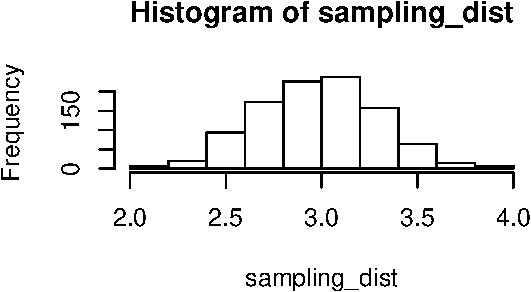
\includegraphics{pdaps_files/figure-latex/sampling-dist-results-1}

For loops are fun, but don't overuse them. Many simple operations are
\textbf{vectorized} and don't require a loop. For example, suppose you
want to take the square of a sequence of numbers. You could use a for
loop \ldots{}

\begin{Shaded}
\begin{Highlighting}[]
\NormalTok{input <-}\StringTok{ }\KeywordTok{c}\NormalTok{(}\DecValTok{1}\NormalTok{, }\DecValTok{3}\NormalTok{, }\DecValTok{7}\NormalTok{, }\DecValTok{29}\NormalTok{)}
\NormalTok{output <-}\StringTok{ }\KeywordTok{rep}\NormalTok{(}\OtherTok{NA}\NormalTok{, }\KeywordTok{length}\NormalTok{(input))}

\NormalTok{for (i in }\DecValTok{1}\NormalTok{:}\KeywordTok{length}\NormalTok{(input)) \{}
    \NormalTok{output[i] <-}\StringTok{ }\NormalTok{input[i]^}\DecValTok{2}
\NormalTok{\}}

\NormalTok{output}
\end{Highlighting}
\end{Shaded}

\begin{verbatim}
## [1]   1   9  49 841
\end{verbatim}

\ldots{} but it's faster (in terms of computational speed) and easier to
just take advantage of vectorization:

\begin{Shaded}
\begin{Highlighting}[]
\NormalTok{input^}\DecValTok{2}
\end{Highlighting}
\end{Shaded}

\begin{verbatim}
## [1]   1   9  49 841
\end{verbatim}

Another useful piece of control flow is \textbf{if/else statements}.
These check a logical condition---an expression whose value is
\texttt{TRUE} or \texttt{FALSE}---and run different code depending on
the value of the expression. (You may want to catch up on the comparison
operators: \texttt{==}, \texttt{\textgreater{}},
\texttt{\textgreater{}=}, \texttt{\textless{}}, \texttt{\textless{}=},
etc.)

Let's edit the \texttt{pois\_mean} function to allow us to calculate the
median instead of the mean. We'll add a second argument to the function,
and implement the option using an if/else statement.

\begin{Shaded}
\begin{Highlighting}[]
\NormalTok{pois_mean <-}\StringTok{ }\NormalTok{function(n_obs, }\DataTypeTok{use_median =} \OtherTok{FALSE}\NormalTok{) \{}
    \NormalTok{samp <-}\StringTok{ }\KeywordTok{rpois}\NormalTok{(n_obs, }\DataTypeTok{lambda =} \DecValTok{3}\NormalTok{)}
    \NormalTok{if (use_median) \{}
        \NormalTok{ans <-}\StringTok{ }\KeywordTok{median}\NormalTok{(samp)}
    \NormalTok{\} else \{}
        \NormalTok{ans <-}\StringTok{ }\KeywordTok{mean}\NormalTok{(samp)}
    \NormalTok{\}}
    \KeywordTok{return}\NormalTok{(ans)}
\NormalTok{\}}
\end{Highlighting}
\end{Shaded}

A couple of things to notice about the structure of the function. We use
a comma to separate multiple function arguments. Also, we've specified
\texttt{FALSE} as the \emph{default} for the \texttt{use\_median}
argument. If we call the function without explicitly specifying a value
for \texttt{use\_median}, the function sets it to \texttt{FALSE}.

\begin{Shaded}
\begin{Highlighting}[]
\KeywordTok{pois_mean}\NormalTok{(}\DataTypeTok{n_obs =} \DecValTok{9}\NormalTok{)}
\end{Highlighting}
\end{Shaded}

\begin{verbatim}
## [1] 3.7778
\end{verbatim}

\begin{Shaded}
\begin{Highlighting}[]
\KeywordTok{pois_mean}\NormalTok{(}\DataTypeTok{n_obs =} \DecValTok{9}\NormalTok{, }\DataTypeTok{use_median =} \OtherTok{TRUE}\NormalTok{)}
\end{Highlighting}
\end{Shaded}

\begin{verbatim}
## [1] 2
\end{verbatim}

\begin{Shaded}
\begin{Highlighting}[]
\KeywordTok{pois_mean}\NormalTok{(}\DataTypeTok{n_obs =} \DecValTok{9}\NormalTok{, }\DataTypeTok{use_median =} \OtherTok{FALSE}\NormalTok{)}
\end{Highlighting}
\end{Shaded}

\begin{verbatim}
## [1] 2.6667
\end{verbatim}

There is a vectorized version of if/else statements called, naturally,
the \texttt{ifelse} function. This function takes three arguments, each
a vector of the same length: (1) a logical condition, (2) an output
value if the condition is \texttt{TRUE}, (3) an output value if the
condition is \texttt{FALSE}.

\begin{Shaded}
\begin{Highlighting}[]
\NormalTok{x <-}\StringTok{ }\DecValTok{1}\NormalTok{:}\DecValTok{10}
\NormalTok{big_x <-}\StringTok{ }\NormalTok{x *}\StringTok{ }\DecValTok{100}
\NormalTok{small_x <-}\StringTok{ }\NormalTok{x *}\StringTok{ }\NormalTok{-}\DecValTok{100}

\KeywordTok{ifelse}\NormalTok{(x >}\StringTok{ }\DecValTok{5}\NormalTok{, big_x, small_x)}
\end{Highlighting}
\end{Shaded}

\begin{verbatim}
##  [1] -100 -200 -300 -400 -500  600  700  800
##  [9]  900 1000
\end{verbatim}

Functions, for loops, and if/else statements are just a few of the
useful tools for programming in R.\footnote{Others include the
  \texttt{replicate} function, the \texttt{apply} family of functions
  (\texttt{sapply}, \texttt{lapply}, \texttt{tapply}, \texttt{mapply},
  \ldots{}), the \textbf{foreach} package, the \textbf{purrr} package,
  just to name a few of the most useful off the top of my head.} But
even these simple tools are enough to allow you to do much more at scale
than you could with a copy-paste philosophy.

\chapter{Working with Data}\label{data}

\emph{Some material in this chapter is adapted from notes
\href{http://mdilorenzo.github.io}{Matt DiLorenzo} wrote for the Spring
2016 session of PSCI 8357.}

Let me repeat something I said last week. In your careers as social
scientists, starting with your dissertation research---if not
earlier---you will probably spend more time collecting, merging, and
cleaning data than you will on statistical analysis. So it's worth
taking some time to learn how to do this well.

Best practices for data management can be summarized in a single
sentence: \emph{Record and document everything you do to the data.}

The first corollary of this principle is that raw data is sacrosanct.
You should never edit raw data ``in place''. Once you download the raw
data file, that file should never change.\footnote{Even if it's data you
  collected yourself, that data should still have a ``canonical''
  representation that never gets overwritten. See \citet{Leek:2015uw}
  for more on distributing your own data.}

In almost any non-trivial analysis, the ``final'' data---the format you
plug into your analysis---will differ significantly from the raw data.
It may consist of information merged from multiple sources. The
variables may have been transformed, aggregated, or otherwise altered.
The unit of observation may even differ from the original source. You
must document every one of these changes, so that another researcher
working from the exact same raw data will end up with the exact same
final data.

The most sensible way to achieve this level of reproducibility is to do
all of your data merging and cleaning in a script. In other words, no
going into Excel and mucking around manually. Like any other piece of
your analysis, your pipeline from raw data to final data should follow
the \protect\hyperlink{programming}{principles of programming} that we
discussed last week.

Luckily for you,\footnote{But not for me, because these tools didn't
  exist when I was a PhD student. Also, get off my lawn!} the
\textbf{tidyverse} suite of R packages (including \textbf{dplyr},
\textbf{tidyr}, and others) makes it easy to script your ``data
pipeline''. We'll begin by loading the package.

\begin{Shaded}
\begin{Highlighting}[]
\KeywordTok{library}\NormalTok{(}\StringTok{"tidyverse"}\NormalTok{)}
\end{Highlighting}
\end{Shaded}

\section{Loading}\label{loading}

The first step in working with data is to acquire some data. Depending
on the nature of your research, you will be getting some or all of your
data from sources available online. When you download data from online
repositories, you should keep track of where you got it from. The best
way to do so is---you guessed it---to script your data acquisition.

The R function \texttt{download.file()} is the easiest way to download
files from URLs from within R. Just specify where you're getting the
file from and where you want it to go. For the examples today, we'll use
an ``untidied'' version of the World Development Indicators data from
the World Bank that I've posted to my website.

\begin{Shaded}
\begin{Highlighting}[]
\KeywordTok{download.file}\NormalTok{(}\DataTypeTok{url =} \StringTok{"http://bkenkel.com/data/untidy-data.csv"}\NormalTok{, }
    \DataTypeTok{destfile =} \StringTok{"my-untidy-data.csv"}\NormalTok{)}
\end{Highlighting}
\end{Shaded}

Once you've got the file stored locally, use the utilities from the
\textbf{readr} package (part of \textbf{tidyverse}) to read it into R as
a data frame.\footnote{More precisely, the \textbf{readr} functions
  produce output of class \texttt{"tbl\_df"} (pronounced ``tibble
  diff,'' I'm told), which are like data frames but better. See
  \texttt{help(package\ =\ "tibble")} for what can be done with
  \texttt{tbl\_df}s.} We have a CSV file, so we will use
\texttt{read\_csv}. See \texttt{help(package\ =\ "readr")} for other
possibilities.

\begin{Shaded}
\begin{Highlighting}[]
\NormalTok{untidy_data <-}\StringTok{ }\KeywordTok{read_csv}\NormalTok{(}\DataTypeTok{file =} \StringTok{"my-untidy-data.csv"}\NormalTok{)}
\end{Highlighting}
\end{Shaded}

\begin{verbatim}
## Parsed with column specification:
## cols(
##   country = col_character(),
##   gdp.2005 = col_double(),
##   gdp.2006 = col_double(),
##   gdp.2007 = col_double(),
##   gdp.2008 = col_double(),
##   pop.2005 = col_double(),
##   pop.2006 = col_double(),
##   pop.2007 = col_double(),
##   pop.2008 = col_double(),
##   unemp.2005 = col_double(),
##   unemp.2006 = col_double(),
##   unemp.2007 = col_double(),
##   unemp.2008 = col_double()
## )
\end{verbatim}

Remember that each column of a data frame might be a different type, or
more formally \emph{class}, of object. \texttt{read\_csv} and its ilk
try to guess the type of data each column contains: character, integer,
decimal number (``double'' in programming-speak), or something else. The
readout above tells you what guesses it made. If it gets something
wrong---say, reading a column as numbers that ought to be
characters---you can use the \texttt{col\_types} argument to set it
straight.

FYI, you could also run \texttt{read\_csv()} directly on a URL, as in:

\begin{Shaded}
\begin{Highlighting}[]
\KeywordTok{read_csv}\NormalTok{(}\StringTok{"http://bkenkel.com/data/untidy-data.csv"}\NormalTok{)}
\end{Highlighting}
\end{Shaded}

However, in analyses intended for publication, it's usually preferable
to download and save the raw data. What's stored at a URL might change
or disappear, and you'll need to have a hard copy of the raw data for
replication purposes.

Now let's take a look at the data we've just loaded in.

\begin{Shaded}
\begin{Highlighting}[]
\KeywordTok{head}\NormalTok{(untidy_data)}
\end{Highlighting}
\end{Shaded}

\begin{verbatim}
## # A tibble: 6 × 13
##   country gdp.2005 gdp.2006 gdp.2007
##     <chr>    <dbl>    <dbl>    <dbl>
## 1      AD   3.8423   4.0184   4.0216
## 2      AE 253.9655 278.9489 287.8318
## 3      AF   9.7630  10.3052  11.7212
## 4      AG   1.1190   1.2687   1.3892
## 5      AL   9.2684   9.7718  10.3483
## 6      AM   7.6678   8.6797   9.8731
## # ... with 9 more variables: gdp.2008 <dbl>,
## #   pop.2005 <dbl>, pop.2006 <dbl>,
## #   pop.2007 <dbl>, pop.2008 <dbl>,
## #   unemp.2005 <dbl>, unemp.2006 <dbl>,
## #   unemp.2007 <dbl>, unemp.2008 <dbl>
\end{verbatim}

We have a \texttt{country} variable giving country abbreviations. The
other variables are numerical values: the country's GDP in 2005, 2006,
2007, and 2008; then the same for population and unemployment. Let's get
this into a format we could use for analysis.

\section{Tidying}\label{tidying}

\citet{Wickham:2014vp} outlines three qualities that make data ``tidy'':

\begin{enumerate}
\def\labelenumi{\arabic{enumi}.}
\tightlist
\item
  Each variable forms a column.
\item
  Each observation forms a row.
\item
  Each type of observational unit forms a table.
\end{enumerate}

For one thing, this means that whether a dataset is tidy or not
depends---at least in part (some data collections are messy from any
angle)---on the purpose it's being analyzed for.

Each row of \texttt{untidy\_data} is a country. In observational studies
in comparative politics and international relations, more commonly the
unit of observation is the country-year.\footnote{Insert lame joke about
  how Americanists haven't heard of other countries. But, seriously, if
  you're confused because you haven't heard of other countries, just
  think of ``state-years''.} How can we take \texttt{untidy\_data} and
easily make it into country-year data?

We'll use the \textbf{tidyr} package (again, part of \textbf{tidyverse})
to clean up this data. The biggest problem right now is that each
column, besides the country identifier, really encodes two pieces of
information: the year of observation and the variable being observed. To
deal with this, we'll have to first transform the data from one untidy
format to another. We're going to use the \texttt{gather()} function to
make each row a country-year-variable.

What \texttt{gather()} does is make a row for each entry from a set of
columns. It's probably easiest to understand it by seeing it in
practice:

\begin{Shaded}
\begin{Highlighting}[]
\NormalTok{long_data <-}\StringTok{ }\KeywordTok{gather}\NormalTok{(untidy_data, }\DataTypeTok{key =} \NormalTok{variable, }
    \DataTypeTok{value =} \NormalTok{number, gdp}\FloatTok{.2005}\NormalTok{:unemp}\FloatTok{.2008}\NormalTok{)}
\KeywordTok{head}\NormalTok{(long_data)}
\end{Highlighting}
\end{Shaded}

\begin{verbatim}
## # A tibble: 6 × 3
##   country variable   number
##     <chr>    <chr>    <dbl>
## 1      AD gdp.2005   3.8423
## 2      AE gdp.2005 253.9655
## 3      AF gdp.2005   9.7630
## 4      AG gdp.2005   1.1190
## 5      AL gdp.2005   9.2684
## 6      AM gdp.2005   7.6678
\end{verbatim}

With the first argument, we told \texttt{gather()} to use the
\texttt{untidy\_data} data frame. With the last argument, we told it the
set of columns to ``gather'' together into a single column. The
\texttt{key} column specifies the name of the variable to store the
``key'' (original column name) in, and the \texttt{value} column
specifies the name of the variable to store the associated value. For
example, the second row of \texttt{long\_data} encodes what we
previously saw as the \texttt{gdp.2005} column of \texttt{untidy\_data}.

Now we have a new problem, which is that \texttt{variable} encodes two
pieces of information: the variable and the year of its observation.
\textbf{tidyr} provides the \texttt{separate()} function to solve that,
splitting a single variable into two.

\begin{Shaded}
\begin{Highlighting}[]
\NormalTok{long_data <-}\StringTok{ }\KeywordTok{separate}\NormalTok{(long_data, }\DataTypeTok{col =} \NormalTok{variable, }
    \DataTypeTok{into =} \KeywordTok{c}\NormalTok{(}\StringTok{"var"}\NormalTok{, }\StringTok{"year"}\NormalTok{))}
\KeywordTok{head}\NormalTok{(long_data)}
\end{Highlighting}
\end{Shaded}

\begin{verbatim}
## # A tibble: 6 × 4
##   country   var  year   number
##     <chr> <chr> <chr>    <dbl>
## 1      AD   gdp  2005   3.8423
## 2      AE   gdp  2005 253.9655
## 3      AF   gdp  2005   9.7630
## 4      AG   gdp  2005   1.1190
## 5      AL   gdp  2005   9.2684
## 6      AM   gdp  2005   7.6678
\end{verbatim}

So now we have country-year-variable data, with the year and variable
conveniently stored in different columns. To turn this into country-year
data, we can use the \texttt{spread()} function, which is like the
inverse of \texttt{gather()}. \texttt{spread()} takes a key column and a
value column, and turns each different key into a column of its own.

\begin{Shaded}
\begin{Highlighting}[]
\NormalTok{clean_data <-}\StringTok{ }\KeywordTok{spread}\NormalTok{(long_data, }\DataTypeTok{key =} \NormalTok{var, }\DataTypeTok{value =} \NormalTok{number)}
\KeywordTok{head}\NormalTok{(clean_data)}
\end{Highlighting}
\end{Shaded}

\begin{verbatim}
## # A tibble: 6 × 5
##   country  year      gdp      pop unemp
##     <chr> <chr>    <dbl>    <dbl> <dbl>
## 1      AD  2005   3.8423 0.081223    NA
## 2      AD  2006   4.0184 0.083373    NA
## 3      AD  2007   4.0216 0.084878    NA
## 4      AD  2008   3.6759 0.085616    NA
## 5      AE  2005 253.9655 4.481976   3.1
## 6      AE  2006 278.9489 5.171255   3.3
\end{verbatim}

When using \texttt{spread()} on data that you didn't previously
\texttt{gather()}, be sure to set the \texttt{fill} argument to tell it
how to fill in empty cells. A simple example:

\begin{Shaded}
\begin{Highlighting}[]
\NormalTok{test_data}
\end{Highlighting}
\end{Shaded}

\begin{verbatim}
## # A tibble: 3 × 3
##        id     k     v
##     <chr> <chr> <dbl>
## 1 brenton     a    10
## 2 brenton     b    20
## 3 patrick     b     5
\end{verbatim}

\begin{Shaded}
\begin{Highlighting}[]
\KeywordTok{spread}\NormalTok{(test_data, }\DataTypeTok{key =} \NormalTok{k, }\DataTypeTok{value =} \NormalTok{v)}
\end{Highlighting}
\end{Shaded}

\begin{verbatim}
## # A tibble: 2 × 3
##        id     a     b
## *   <chr> <dbl> <dbl>
## 1 brenton    10    20
## 2 patrick    NA     5
\end{verbatim}

\begin{Shaded}
\begin{Highlighting}[]
\KeywordTok{spread}\NormalTok{(test_data, }\DataTypeTok{key =} \NormalTok{k, }\DataTypeTok{value =} \NormalTok{v, }\DataTypeTok{fill =} \DecValTok{100}\NormalTok{)}
\end{Highlighting}
\end{Shaded}

\begin{verbatim}
## # A tibble: 2 × 3
##        id     a     b
## *   <chr> <dbl> <dbl>
## 1 brenton    10    20
## 2 patrick   100     5
\end{verbatim}

One more important note on \textbf{tidyverse} semantics. It includes a
fabulous feature called the \emph{pipe}, \texttt{\%\textgreater{}\%},
which makes it easy to string together a truly mind-boggling number of
commands.

In pipe syntax, \texttt{x\ \%\textgreater{}\%\ f()} is equivalent to
\texttt{f(x)}. That seems like a wasteful and confusing way to write
\texttt{f(x)}, and it is. But if you want to string together a bunch of
commands, it's much easier to comprehend

\begin{Shaded}
\begin{Highlighting}[]
\NormalTok{x %>%}\StringTok{ }\KeywordTok{f}\NormalTok{() %>%}\StringTok{ }\KeywordTok{g}\NormalTok{() %>%}\StringTok{ }\KeywordTok{h}\NormalTok{() %>%}\StringTok{ }\KeywordTok{i}\NormalTok{()}
\end{Highlighting}
\end{Shaded}

than \texttt{i(h(g(f(x))))}.

You can pass function arguments using the pipe too. For example,
\texttt{f(x,\ bear\ =\ "moose")} is equivalent to
\texttt{x\ \%\textgreater{}\%\ f(bear\ =\ "moose")}.

The key thing about the \textbf{tidyverse} functions is that each of
them takes a data frame as its first argument, and returns a data frame
as its output. This makes them highly amenable to piping. For example,
we can combine all three steps of our tidying above with a single
command, thanks to the pipe:\footnote{If you are reading the PDF copy of
  these notes (i.e., the ones I hand out in class), the line breaks are
  eliminated, making the piped commands rather hard to read. I am
  working on fixing this. For now, you may find the online notes at
  \url{http://bkenkel.com/pdaps} easier to follow.}

\begin{Shaded}
\begin{Highlighting}[]
\NormalTok{untidy_data %>%}\StringTok{ }\KeywordTok{gather}\NormalTok{(}\DataTypeTok{key =} \NormalTok{variable, }\DataTypeTok{value =} \NormalTok{number, }
    \NormalTok{gdp}\FloatTok{.2005}\NormalTok{:unemp}\FloatTok{.2008}\NormalTok{) %>%}\StringTok{ }\KeywordTok{separate}\NormalTok{(}\DataTypeTok{col =} \NormalTok{variable, }
    \DataTypeTok{into =} \KeywordTok{c}\NormalTok{(}\StringTok{"var"}\NormalTok{, }\StringTok{"year"}\NormalTok{)) %>%}\StringTok{ }\KeywordTok{spread}\NormalTok{(}\DataTypeTok{key =} \NormalTok{var, }
    \DataTypeTok{value =} \NormalTok{number)}
\end{Highlighting}
\end{Shaded}

\begin{verbatim}
## # A tibble: 860 × 5
##   country  year      gdp      pop unemp
## *   <chr> <chr>    <dbl>    <dbl> <dbl>
## 1      AD  2005   3.8423 0.081223    NA
## 2      AD  2006   4.0184 0.083373    NA
## 3      AD  2007   4.0216 0.084878    NA
## 4      AD  2008   3.6759 0.085616    NA
## 5      AE  2005 253.9655 4.481976   3.1
## # ... with 855 more rows
\end{verbatim}

Without the pipe, if we wanted to run all those commands together, we
would have to write:

\begin{Shaded}
\begin{Highlighting}[]
\KeywordTok{spread}\NormalTok{(}\KeywordTok{separate}\NormalTok{(}\KeywordTok{gather}\NormalTok{(untidy_data, }\DataTypeTok{key =} \NormalTok{variable, }
    \DataTypeTok{value =} \NormalTok{number, gdp}\FloatTok{.2005}\NormalTok{:unemp}\FloatTok{.2008}\NormalTok{), }\DataTypeTok{col =} \NormalTok{variable, }
    \DataTypeTok{into =} \KeywordTok{c}\NormalTok{(}\StringTok{"var"}\NormalTok{, }\StringTok{"year"}\NormalTok{)), }\DataTypeTok{key =} \NormalTok{var, }\DataTypeTok{value =} \NormalTok{number)}
\end{Highlighting}
\end{Shaded}

Sad!

\section{Transforming and
Aggregating}\label{transforming-and-aggregating}

Tidying the data usually isn't the end of the process. If you want to
perform further calculations on the raw, that's where the tools in
\textbf{dplyr} (part of, you guessed it, the \textbf{tidyverse}) come
in.

Perhaps the simplest \textbf{dplyr} function (or ``verb'', as the R
hipsters would say) is \texttt{rename()}, which lets you rename columns.

\begin{Shaded}
\begin{Highlighting}[]
\NormalTok{clean_data %>%}\StringTok{ }\KeywordTok{rename}\NormalTok{(}\DataTypeTok{gross_domestic_product =} \NormalTok{gdp)}
\end{Highlighting}
\end{Shaded}

\begin{verbatim}
## # A tibble: 860 × 5
##   country  year gross_domestic_product
## *   <chr> <chr>                  <dbl>
## 1      AD  2005                 3.8423
## 2      AD  2006                 4.0184
## 3      AD  2007                 4.0216
## 4      AD  2008                 3.6759
## 5      AE  2005               253.9655
## # ... with 855 more rows, and 2 more
## #   variables: pop <dbl>, unemp <dbl>
\end{verbatim}

The \textbf{dplyr} functions, like the vast majority of R functions, do
not modify their inputs. In other words, running \texttt{rename()} on
\texttt{clean\_data} will return a renamed copy of \texttt{clean\_data},
but won't overwrite the original.

\begin{Shaded}
\begin{Highlighting}[]
\NormalTok{clean_data}
\end{Highlighting}
\end{Shaded}

\begin{verbatim}
## # A tibble: 860 × 5
##   country  year      gdp      pop unemp
## *   <chr> <chr>    <dbl>    <dbl> <dbl>
## 1      AD  2005   3.8423 0.081223    NA
## 2      AD  2006   4.0184 0.083373    NA
## 3      AD  2007   4.0216 0.084878    NA
## 4      AD  2008   3.6759 0.085616    NA
## 5      AE  2005 253.9655 4.481976   3.1
## # ... with 855 more rows
\end{verbatim}

If you wanted to make the change stick, you would have to run:

\begin{Shaded}
\begin{Highlighting}[]
\NormalTok{clean_data <-}\StringTok{ }\NormalTok{clean_data %>%}\StringTok{ }\KeywordTok{rename}\NormalTok{(}\DataTypeTok{gross_domestic_product =} \NormalTok{gdp)}
\end{Highlighting}
\end{Shaded}

\texttt{select()} lets you keep a couple of columns and drop all the
others. Or vice versa if you use minus signs.

\begin{Shaded}
\begin{Highlighting}[]
\NormalTok{clean_data %>%}\StringTok{ }\KeywordTok{select}\NormalTok{(country, gdp)}
\end{Highlighting}
\end{Shaded}

\begin{verbatim}
## # A tibble: 860 × 2
##   country      gdp
## *   <chr>    <dbl>
## 1      AD   3.8423
## 2      AD   4.0184
## 3      AD   4.0216
## 4      AD   3.6759
## 5      AE 253.9655
## # ... with 855 more rows
\end{verbatim}

\begin{Shaded}
\begin{Highlighting}[]
\NormalTok{clean_data %>%}\StringTok{ }\KeywordTok{select}\NormalTok{(-pop)}
\end{Highlighting}
\end{Shaded}

\begin{verbatim}
## # A tibble: 860 × 4
##   country  year      gdp unemp
## *   <chr> <chr>    <dbl> <dbl>
## 1      AD  2005   3.8423    NA
## 2      AD  2006   4.0184    NA
## 3      AD  2007   4.0216    NA
## 4      AD  2008   3.6759    NA
## 5      AE  2005 253.9655   3.1
## # ... with 855 more rows
\end{verbatim}

\texttt{mutate()} lets you create new variables that are transformations
of old ones.

\begin{Shaded}
\begin{Highlighting}[]
\NormalTok{clean_data %>%}\StringTok{ }\KeywordTok{mutate}\NormalTok{(}\DataTypeTok{gdppc =} \NormalTok{gdp/pop, }\DataTypeTok{log_gdppc =} \KeywordTok{log}\NormalTok{(gdppc))}
\end{Highlighting}
\end{Shaded}

\begin{verbatim}
## # A tibble: 860 × 7
##   country  year      gdp      pop unemp
##     <chr> <chr>    <dbl>    <dbl> <dbl>
## 1      AD  2005   3.8423 0.081223    NA
## 2      AD  2006   4.0184 0.083373    NA
## 3      AD  2007   4.0216 0.084878    NA
## 4      AD  2008   3.6759 0.085616    NA
## 5      AE  2005 253.9655 4.481976   3.1
## # ... with 855 more rows, and 2 more
## #   variables: gdppc <dbl>, log_gdppc <dbl>
\end{verbatim}

\texttt{filter()} cuts down the data according to the logical
condition(s) you specify.

\begin{Shaded}
\begin{Highlighting}[]
\NormalTok{clean_data %>%}\StringTok{ }\KeywordTok{filter}\NormalTok{(year ==}\StringTok{ }\DecValTok{2006}\NormalTok{)}
\end{Highlighting}
\end{Shaded}

\begin{verbatim}
## # A tibble: 215 × 5
##   country  year      gdp       pop unemp
##     <chr> <chr>    <dbl>     <dbl> <dbl>
## 1      AD  2006   4.0184  0.083373    NA
## 2      AE  2006 278.9489  5.171255   3.3
## 3      AF  2006  10.3052 25.183615   8.8
## 4      AG  2006   1.2687  0.083467    NA
## 5      AL  2006   9.7718  2.992547  12.4
## # ... with 210 more rows
\end{verbatim}

\texttt{summarise()} calculates summaries of the data. For example,
let's find the maximum unemployment rate.

\begin{Shaded}
\begin{Highlighting}[]
\NormalTok{clean_data %>%}\StringTok{ }\KeywordTok{summarise}\NormalTok{(}\DataTypeTok{max_unemp =} \KeywordTok{max}\NormalTok{(unemp, }
    \DataTypeTok{na.rm =} \OtherTok{TRUE}\NormalTok{))}
\end{Highlighting}
\end{Shaded}

\begin{verbatim}
## # A tibble: 1 × 1
##   max_unemp
##       <dbl>
## 1      37.6
\end{verbatim}

This seems sort of useless, until you combine it with the
\texttt{group\_by()} function. If you group the data before
\texttt{summarise}-ing it, you'll calculate a separate summary for each
group. For example, let's calculate the maximum unemployment rate for
each year in the data.

\begin{Shaded}
\begin{Highlighting}[]
\NormalTok{clean_data %>%}\StringTok{ }\KeywordTok{group_by}\NormalTok{(year) %>%}\StringTok{ }\KeywordTok{summarise}\NormalTok{(}\DataTypeTok{max_unemp =} \KeywordTok{max}\NormalTok{(unemp, }
    \DataTypeTok{na.rm =} \OtherTok{TRUE}\NormalTok{))}
\end{Highlighting}
\end{Shaded}

\begin{verbatim}
## # A tibble: 4 × 2
##    year max_unemp
##   <chr>     <dbl>
## 1  2005      37.3
## 2  2006      36.0
## 3  2007      34.9
## 4  2008      37.6
\end{verbatim}

\texttt{summarise()} produces a ``smaller'' data frame than the
input---one row per group. If you want to do something similar, but
preserving the structure of the original data, use \texttt{mutate} in
combination with \texttt{group\_by}.

\begin{Shaded}
\begin{Highlighting}[]
\NormalTok{clean_data %>%}\StringTok{ }\KeywordTok{group_by}\NormalTok{(year) %>%}\StringTok{ }\KeywordTok{mutate}\NormalTok{(}\DataTypeTok{max_unemp =} \KeywordTok{max}\NormalTok{(unemp, }
    \DataTypeTok{na.rm =} \OtherTok{TRUE}\NormalTok{), }\DataTypeTok{unemp_over_max =} \NormalTok{unemp/max_unemp) %>%}\StringTok{ }
\StringTok{    }\KeywordTok{select}\NormalTok{(country, year, }\KeywordTok{contains}\NormalTok{(}\StringTok{"unemp"}\NormalTok{))}
\end{Highlighting}
\end{Shaded}

\begin{verbatim}
## Source: local data frame [860 x 5]
## Groups: year [4]
## 
##   country  year unemp max_unemp
##     <chr> <chr> <dbl>     <dbl>
## 1      AD  2005    NA      37.3
## 2      AD  2006    NA      36.0
## 3      AD  2007    NA      34.9
## 4      AD  2008    NA      37.6
## 5      AE  2005   3.1      37.3
## # ... with 855 more rows, and 1 more
## #   variables: unemp_over_max <dbl>
\end{verbatim}

This gives us back the original data, but with a \texttt{max\_unemp}
variable recording the highest unemployment level that year. We can then
calculate each individual country's unemployment as a percentage of the
maximum. Whether grouped \texttt{mutate} or \texttt{summarise} is better
depends, of course, on the purpose and structure of your analysis.

Notice how I selected all of the unemployment-related columns with
\texttt{contains("unemp")}. See \texttt{?select\_helpers} for a full
list of helpful functions like this for \texttt{select}-ing variables.

\section{Merging}\label{merging}

Only rarely will you be lucky enough to draw all your data from a single
source. More often, you'll be merging together data from multiple
sources.

The key to merging data from separate tables is to have consistent
identifiers across tables. For example, if you run an experiment, you
might have demographic data on each subject in one table, and each
subject's response to each treatment in another table. Naturally, you'll
want to have a subject identifier that ``links'' the records across
tables, as in the following hypothetical example.

\begin{Shaded}
\begin{Highlighting}[]
\NormalTok{subject_data}
\end{Highlighting}
\end{Shaded}

\begin{verbatim}
## # A tibble: 3 × 4
##      id gender loves_bernie does_yoga
##   <dbl>  <chr>        <chr>     <chr>
## 1  1001   male          yes        no
## 2  1002 female           no       yes
## 3  1003   male           no        no
\end{verbatim}

\begin{Shaded}
\begin{Highlighting}[]
\NormalTok{subject_response_data}
\end{Highlighting}
\end{Shaded}

\begin{verbatim}
## # A tibble: 6 × 3
##      id treatment response
##   <dbl>     <chr>    <chr>
## 1  1001 read_book      sad
## 2  1001  watch_tv      sad
## 3  1002 read_book    happy
## 4  1002  watch_tv      sad
## 5  1003 read_book      sad
## 6  1003  watch_tv    happy
\end{verbatim}

Let's practice merging data with our cleaned-up country-year data. We'll
take two datasets from my website: a country-level dataset with
latitudes and longitudes, and a country-year--level dataset with
inflation over time.

\begin{Shaded}
\begin{Highlighting}[]
\NormalTok{latlong_data <-}\StringTok{ }\KeywordTok{read_csv}\NormalTok{(}\StringTok{"http://bkenkel.com/data/latlong.csv"}\NormalTok{)}
\NormalTok{latlong_data}
\end{Highlighting}
\end{Shaded}

\begin{verbatim}
## # A tibble: 245 × 3
##   country latitude longitude
##     <chr>    <dbl>     <dbl>
## 1      AD   42.546    1.6016
## 2      AE   23.424   53.8478
## 3      AF   33.939   67.7100
## 4      AG   17.061  -61.7964
## 5      AI   18.221  -63.0686
## # ... with 240 more rows
\end{verbatim}

\begin{Shaded}
\begin{Highlighting}[]
\NormalTok{inflation_data <-}\StringTok{ }\KeywordTok{read_csv}\NormalTok{(}\StringTok{"http://bkenkel.com/data/inflation.csv"}\NormalTok{)}
\NormalTok{inflation_data}
\end{Highlighting}
\end{Shaded}

\begin{verbatim}
## # A tibble: 1,070 × 3
##   country  year inflation
##     <chr> <int>     <dbl>
## 1      AD  2004        NA
## 2      AD  2005        NA
## 3      AD  2006        NA
## 4      AD  2007        NA
## 5      AD  2008        NA
## # ... with 1,065 more rows
\end{verbatim}

For your convenience, both of these datasets use the same two-letter
country naming scheme as the original data. Unfortunately, out in the
real world, data from different sources often use incommensurate naming
schemes. Converting from one naming scheme to another is part of the
data cleaning process, and it requires careful attention.

\textbf{dplyr} contains various \texttt{\_join()} functions for merging.
Each of these take as arguments the two data frames to merge, plus the
names of the identifier variables to merge them on. The one I use most
often is \texttt{left\_join()}, which keeps every row from the first
(``left'') data frame and merges in the columns from the second
(``right'') data frame.

For example, let's merge the latitude and longitude data for each
country into \texttt{clean\_data}.

\begin{Shaded}
\begin{Highlighting}[]
\KeywordTok{left_join}\NormalTok{(clean_data, latlong_data, }\DataTypeTok{by =} \StringTok{"country"}\NormalTok{)}
\end{Highlighting}
\end{Shaded}

\begin{verbatim}
## # A tibble: 860 × 7
##   country  year      gdp      pop unemp
##     <chr> <chr>    <dbl>    <dbl> <dbl>
## 1      AD  2005   3.8423 0.081223    NA
## 2      AD  2006   4.0184 0.083373    NA
## 3      AD  2007   4.0216 0.084878    NA
## 4      AD  2008   3.6759 0.085616    NA
## 5      AE  2005 253.9655 4.481976   3.1
## # ... with 855 more rows, and 2 more
## #   variables: latitude <dbl>,
## #   longitude <dbl>
\end{verbatim}

Since \texttt{latlong\_data} is country-level, the value is the same for
each year. So the merged data contains redundant information. This is
one reason to store data observed at different levels in different
tables---with redundant observations, it is easier to make errors yet
harder to catch them and fix them.

We can also merge data when the identifier is stored across multiple
columns, as in the case of our country-year data. But first, a technical
note.\footnote{This won't be the case if you got \texttt{clean\_data} by
  loading it in directly from \texttt{clean-data.csv} on my website,
  since \texttt{read\_csv()} will have correctly encoded \texttt{year}
  as an integer.} You might notice that the \texttt{year} column of
\texttt{clean\_data} is labeled \texttt{\textless{}chr\textgreater{}},
as in character data. Yet the \texttt{year} column of
\texttt{inflation\_data} is labeled
\texttt{\textless{}int\textgreater{}}, as in integer data. We can check
that by running \texttt{class()} on each respective column.

\begin{Shaded}
\begin{Highlighting}[]
\KeywordTok{class}\NormalTok{(clean_data$year)}
\end{Highlighting}
\end{Shaded}

\begin{verbatim}
## [1] "character"
\end{verbatim}

\begin{Shaded}
\begin{Highlighting}[]
\KeywordTok{class}\NormalTok{(inflation_data$year)}
\end{Highlighting}
\end{Shaded}

\begin{verbatim}
## [1] "integer"
\end{verbatim}

From R's perspective, the character string \texttt{"1999"} is a very
different thing than the integer number \texttt{1999}. Therefore, if we
try to merge \texttt{clean\_data} and \texttt{inflation\_data} on the
\texttt{year} variable, it will throw an error.

\begin{Shaded}
\begin{Highlighting}[]
\KeywordTok{left_join}\NormalTok{(clean_data, inflation_data, }\DataTypeTok{by =} \KeywordTok{c}\NormalTok{(}\StringTok{"country"}\NormalTok{, }
    \StringTok{"year"}\NormalTok{))}
\end{Highlighting}
\end{Shaded}

\begin{verbatim}
## Error in eval(substitute(expr), envir, enclos): Can't join on 'year' x 'year' because of incompatible types (integer / character)
\end{verbatim}

To fix this, let's use \texttt{mutate()} to convert the \texttt{year}
column of \texttt{clean\_data} to an integer. We probably should have
done this in the first place---after all, having the year encoded as a
character string would have thrown off plotting functions, statistical
functions, or anything else where it would be more natural to treat the
year like a number.

\begin{Shaded}
\begin{Highlighting}[]
\NormalTok{clean_data <-}\StringTok{ }\KeywordTok{mutate}\NormalTok{(clean_data, }\DataTypeTok{year =} \KeywordTok{as.integer}\NormalTok{(year))}
\NormalTok{clean_data}
\end{Highlighting}
\end{Shaded}

\begin{verbatim}
## # A tibble: 860 × 5
##   country  year      gdp      pop unemp
##     <chr> <int>    <dbl>    <dbl> <dbl>
## 1      AD  2005   3.8423 0.081223    NA
## 2      AD  2006   4.0184 0.083373    NA
## 3      AD  2007   4.0216 0.084878    NA
## 4      AD  2008   3.6759 0.085616    NA
## 5      AE  2005 253.9655 4.481976   3.1
## # ... with 855 more rows
\end{verbatim}

Looks the same as before, except with an important difference:
\texttt{year} is now labeled \texttt{\textless{}int\textgreater{}}.

Now we can merge the two datasets together without issue. Notice how we
use a vector in the \texttt{by} argument to specify multiple columns to
merge on.

\begin{Shaded}
\begin{Highlighting}[]
\KeywordTok{left_join}\NormalTok{(clean_data, inflation_data, }\DataTypeTok{by =} \KeywordTok{c}\NormalTok{(}\StringTok{"country"}\NormalTok{, }
    \StringTok{"year"}\NormalTok{))}
\end{Highlighting}
\end{Shaded}

\begin{verbatim}
## # A tibble: 860 × 6
##   country  year      gdp      pop unemp
##     <chr> <int>    <dbl>    <dbl> <dbl>
## 1      AD  2005   3.8423 0.081223    NA
## 2      AD  2006   4.0184 0.083373    NA
## 3      AD  2007   4.0216 0.084878    NA
## 4      AD  2008   3.6759 0.085616    NA
## 5      AE  2005 253.9655 4.481976   3.1
## # ... with 855 more rows, and 1 more
## #   variables: inflation <dbl>
\end{verbatim}

You might remember that \texttt{inflation\_data} contained some
country-years not included in the original data (namely, observations
from 2004). If we want the merged data to use the observations from
\texttt{inflation\_data} rather than \texttt{clean\_data}, we can use
the \texttt{right\_join()} function.

\begin{Shaded}
\begin{Highlighting}[]
\KeywordTok{right_join}\NormalTok{(clean_data, inflation_data, }\DataTypeTok{by =} \KeywordTok{c}\NormalTok{(}\StringTok{"country"}\NormalTok{, }
    \StringTok{"year"}\NormalTok{))}
\end{Highlighting}
\end{Shaded}

\begin{verbatim}
## # A tibble: 1,070 × 6
##   country  year    gdp      pop unemp
##     <chr> <int>  <dbl>    <dbl> <dbl>
## 1      AD  2004     NA       NA    NA
## 2      AD  2005 3.8423 0.081223    NA
## 3      AD  2006 4.0184 0.083373    NA
## 4      AD  2007 4.0216 0.084878    NA
## 5      AD  2008 3.6759 0.085616    NA
## # ... with 1,065 more rows, and 1 more
## #   variables: inflation <dbl>
\end{verbatim}

One last common issue in merging is that the identifier variables have
different names in the two datasets. If it's inconvenient or infeasible
to correct this by renaming the columns in one or the other, you can
specify the \texttt{by} argument as in the following example.

\begin{Shaded}
\begin{Highlighting}[]
\NormalTok{inflation_data <-}\StringTok{ }\KeywordTok{rename}\NormalTok{(inflation_data, }\DataTypeTok{the_country =} \NormalTok{country, }
    \DataTypeTok{the_year =} \NormalTok{year)}
\NormalTok{inflation_data}
\end{Highlighting}
\end{Shaded}

\begin{verbatim}
## # A tibble: 1,070 × 3
##   the_country the_year inflation
##         <chr>    <int>     <dbl>
## 1          AD     2004        NA
## 2          AD     2005        NA
## 3          AD     2006        NA
## 4          AD     2007        NA
## 5          AD     2008        NA
## # ... with 1,065 more rows
\end{verbatim}

\begin{Shaded}
\begin{Highlighting}[]
\KeywordTok{left_join}\NormalTok{(clean_data, inflation_data, }\DataTypeTok{by =} \KeywordTok{c}\NormalTok{(}\DataTypeTok{country =} \StringTok{"the_country"}\NormalTok{, }
    \DataTypeTok{year =} \StringTok{"the_year"}\NormalTok{))}
\end{Highlighting}
\end{Shaded}

\begin{verbatim}
## # A tibble: 860 × 6
##   country  year      gdp      pop unemp
##     <chr> <int>    <dbl>    <dbl> <dbl>
## 1      AD  2005   3.8423 0.081223    NA
## 2      AD  2006   4.0184 0.083373    NA
## 3      AD  2007   4.0216 0.084878    NA
## 4      AD  2008   3.6759 0.085616    NA
## 5      AE  2005 253.9655 4.481976   3.1
## # ... with 855 more rows, and 1 more
## #   variables: inflation <dbl>
\end{verbatim}

\section{Appendix: Creating the Example
Data}\label{appendix-creating-the-example-data}

I used the same tools this chapter introduces to create the untidy data.
I may as well include the code to do it, in case it helps further
illustrate how to use the \textbf{tidyverse} tools (and, as a bonus, the
\textbf{WDI} package for downloading World Development Indicators data).

First I load the necessary packages.

\begin{Shaded}
\begin{Highlighting}[]
\KeywordTok{library}\NormalTok{(}\StringTok{"tidyverse"}\NormalTok{)}
\KeywordTok{library}\NormalTok{(}\StringTok{"WDI"}\NormalTok{)}
\KeywordTok{library}\NormalTok{(}\StringTok{"countrycode"}\NormalTok{)}
\KeywordTok{library}\NormalTok{(}\StringTok{"stringr"}\NormalTok{)}
\end{Highlighting}
\end{Shaded}

Next, I download the relevant WDI data. I used the \texttt{WDIsearch()}
function to locate the appropriate indicator names.

\begin{Shaded}
\begin{Highlighting}[]
\NormalTok{dat_raw <-}\StringTok{ }\KeywordTok{WDI}\NormalTok{(}\DataTypeTok{country =} \StringTok{"all"}\NormalTok{,}
               \DataTypeTok{indicator =} \KeywordTok{c}\NormalTok{(}\StringTok{"NY.GDP.MKTP.KD"}\NormalTok{,  }\CommentTok{# GDP in 2000 USD}
                             \StringTok{"SP.POP.TOTL"}\NormalTok{,     }\CommentTok{# Total population}
                             \StringTok{"SL.UEM.TOTL.ZS"}\NormalTok{), }\CommentTok{# Unemployment rate}
               \DataTypeTok{start =} \DecValTok{2005}\NormalTok{,}
               \DataTypeTok{end =} \DecValTok{2008}\NormalTok{)}

\KeywordTok{head}\NormalTok{(dat_raw)}
\end{Highlighting}
\end{Shaded}

\begin{verbatim}
##   iso2c    country year NY.GDP.MKTP.KD
## 1    1A Arab World 2005     1.6428e+12
## 2    1A Arab World 2006     1.7629e+12
## 3    1A Arab World 2007     1.8625e+12
## 4    1A Arab World 2008     1.9799e+12
## 5    1W      World 2005     5.7703e+13
## 6    1W      World 2006     6.0229e+13
##   SP.POP.TOTL SL.UEM.TOTL.ZS
## 1   313430911        12.1402
## 2   320906736        11.3296
## 3   328766559        10.8961
## 4   336886468        10.5060
## 5  6513959904         6.1593
## 6  6594722462         5.9000
\end{verbatim}

I want to get rid of the aggregates, like the ``Arab World'' and
``World'' we see here. As a rough tack at that, I'm going to exclude
those so-called countries whose ISO codes don't appear in the
\textbf{countrycode} package data.\footnote{\textbf{countrycode} is a
  very useful, albeit imperfect, package for converting between
  different country naming/coding schemes.}

\begin{Shaded}
\begin{Highlighting}[]
\NormalTok{dat_countries <-}\StringTok{ }\NormalTok{dat_raw %>%}\StringTok{ }\KeywordTok{filter}\NormalTok{(iso2c %in%}\StringTok{ }
\StringTok{    }\NormalTok{countrycode_data$iso2c)}
\end{Highlighting}
\end{Shaded}

Let's check on which countries are left. (I cut it down to max six
characters per country name for printing purposes.)

\begin{Shaded}
\begin{Highlighting}[]
\NormalTok{dat_countries$country %>%}\StringTok{ }\KeywordTok{unique}\NormalTok{() %>%}\StringTok{ }\KeywordTok{str_sub}\NormalTok{(}\DataTypeTok{start =} \DecValTok{1}\NormalTok{, }
    \DataTypeTok{end =} \DecValTok{6}\NormalTok{)}
\end{Highlighting}
\end{Shaded}

\begin{verbatim}
##   [1] "Andorr" "United" "Afghan" "Antigu"
##   [5] "Albani" "Armeni" "Angola" "Argent"
##   [9] "Americ" "Austri" "Austra" "Aruba" 
##  [13] "Azerba" "Bosnia" "Barbad" "Bangla"
##  [17] "Belgiu" "Burkin" "Bulgar" "Bahrai"
##  [21] "Burund" "Benin"  "Bermud" "Brunei"
##  [25] "Bolivi" "Brazil" "Bahama" "Bhutan"
##  [29] "Botswa" "Belaru" "Belize" "Canada"
##  [33] "Congo," "Centra" "Congo," "Switze"
##  [37] "Cote d" "Chile"  "Camero" "China" 
##  [41] "Colomb" "Costa " "Cuba"   "Cabo V"
##  [45] "Curaca" "Cyprus" "Czech " "German"
##  [49] "Djibou" "Denmar" "Domini" "Domini"
##  [53] "Algeri" "Ecuado" "Estoni" "Egypt,"
##  [57] "Eritre" "Spain"  "Ethiop" "Finlan"
##  [61] "Fiji"   "Micron" "Faroe " "France"
##  [65] "Gabon"  "United" "Grenad" "Georgi"
##  [69] "Ghana"  "Gibral" "Greenl" "Gambia"
##  [73] "Guinea" "Equato" "Greece" "Guatem"
##  [77] "Guam"   "Guinea" "Guyana" "Hong K"
##  [81] "Hondur" "Croati" "Haiti"  "Hungar"
##  [85] "Indone" "Irelan" "Israel" "Isle o"
##  [89] "India"  "Iraq"   "Iran, " "Icelan"
##  [93] "Italy"  "Jamaic" "Jordan" "Japan" 
##  [97] "Kenya"  "Kyrgyz" "Cambod" "Kiriba"
## [101] "Comoro" "St. Ki" "Korea," "Korea,"
## [105] "Kuwait" "Cayman" "Kazakh" "Lao PD"
## [109] "Lebano" "St. Lu" "Liecht" "Sri La"
## [113] "Liberi" "Lesoth" "Lithua" "Luxemb"
## [117] "Latvia" "Libya"  "Morocc" "Monaco"
## [121] "Moldov" "Monten" "St. Ma" "Madaga"
## [125] "Marsha" "Macedo" "Mali"   "Myanma"
## [129] "Mongol" "Macao " "Northe" "Maurit"
## [133] "Malta"  "Maurit" "Maldiv" "Malawi"
## [137] "Mexico" "Malays" "Mozamb" "Namibi"
## [141] "New Ca" "Niger"  "Nigeri" "Nicara"
## [145] "Nether" "Norway" "Nepal"  "Nauru" 
## [149] "New Ze" "Oman"   "Panama" "Peru"  
## [153] "French" "Papua " "Philip" "Pakist"
## [157] "Poland" "Puerto" "West B" "Portug"
## [161] "Palau"  "Paragu" "Qatar"  "Romani"
## [165] "Serbia" "Russia" "Rwanda" "Saudi "
## [169] "Solomo" "Seyche" "Sudan"  "Sweden"
## [173] "Singap" "Sloven" "Slovak" "Sierra"
## [177] "San Ma" "Senega" "Somali" "Surina"
## [181] "South " "Sao To" "El Sal" "Sint M"
## [185] "Syrian" "Swazil" "Turks " "Chad"  
## [189] "Togo"   "Thaila" "Tajiki" "Timor-"
## [193] "Turkme" "Tunisi" "Tonga"  "Turkey"
## [197] "Trinid" "Tuvalu" "Tanzan" "Ukrain"
## [201] "Uganda" "United" "Urugua" "Uzbeki"
## [205] "St. Vi" "Venezu" "Britis" "Virgin"
## [209] "Vietna" "Vanuat" "Samoa"  "Yemen,"
## [213] "South " "Zambia" "Zimbab"
\end{verbatim}

With that out of the way, there's still some cleaning up to do. The
magnitudes of GDP and population are too large, and the variable names
are impenetrable. Also, the \texttt{country} variable, while helpful, is
redundant now that we're satisfied with the list of countries remaining.

\begin{Shaded}
\begin{Highlighting}[]
\NormalTok{dat_countries <-}\StringTok{ }\NormalTok{dat_countries %>%}\StringTok{ }\KeywordTok{select}\NormalTok{(-country) %>%}\StringTok{ }
\StringTok{    }\KeywordTok{rename}\NormalTok{(}\DataTypeTok{gdp =} \NormalTok{NY.GDP.MKTP.KD, }\DataTypeTok{pop =} \NormalTok{SP.POP.TOTL, }
        \DataTypeTok{unemp =} \NormalTok{SL.UEM.TOTL.ZS, }\DataTypeTok{country =} \NormalTok{iso2c) %>%}\StringTok{ }
\StringTok{    }\KeywordTok{mutate}\NormalTok{(}\DataTypeTok{gdp =} \NormalTok{gdp/}\FloatTok{1e+09}\NormalTok{, }\DataTypeTok{pop =} \NormalTok{pop/}\FloatTok{1e+06}\NormalTok{)}

\KeywordTok{head}\NormalTok{(dat_countries)}
\end{Highlighting}
\end{Shaded}

\begin{verbatim}
##   country year      gdp      pop unemp
## 1      AD 2005   3.8423 0.081223    NA
## 2      AD 2006   4.0184 0.083373    NA
## 3      AD 2007   4.0216 0.084878    NA
## 4      AD 2008   3.6759 0.085616    NA
## 5      AE 2005 253.9655 4.481976   3.1
## 6      AE 2006 278.9489 5.171255   3.3
\end{verbatim}

Now I convert the data to ``long'' format.

\begin{Shaded}
\begin{Highlighting}[]
\NormalTok{dat_countries_long <-}\StringTok{ }\NormalTok{dat_countries %>%}\StringTok{ }\KeywordTok{gather}\NormalTok{(}\DataTypeTok{key =} \NormalTok{variable, }
    \DataTypeTok{value =} \NormalTok{value, gdp:unemp)}

\KeywordTok{head}\NormalTok{(dat_countries_long)}
\end{Highlighting}
\end{Shaded}

\begin{verbatim}
##   country year variable    value
## 1      AD 2005      gdp   3.8423
## 2      AD 2006      gdp   4.0184
## 3      AD 2007      gdp   4.0216
## 4      AD 2008      gdp   3.6759
## 5      AE 2005      gdp 253.9655
## 6      AE 2006      gdp 278.9489
\end{verbatim}

I then smush \texttt{variable} and \texttt{year} into a single column,
and drop the individual components.

\begin{Shaded}
\begin{Highlighting}[]
\NormalTok{dat_countries_long <-}\StringTok{ }\NormalTok{dat_countries_long %>%}\StringTok{ }\KeywordTok{mutate}\NormalTok{(}\DataTypeTok{var_year =} \KeywordTok{paste}\NormalTok{(variable, }
    \NormalTok{year, }\DataTypeTok{sep =} \StringTok{"."}\NormalTok{)) %>%}\StringTok{ }\KeywordTok{select}\NormalTok{(-variable, -year)}

\KeywordTok{head}\NormalTok{(dat_countries_long)}
\end{Highlighting}
\end{Shaded}

\begin{verbatim}
##   country    value var_year
## 1      AD   3.8423 gdp.2005
## 2      AD   4.0184 gdp.2006
## 3      AD   4.0216 gdp.2007
## 4      AD   3.6759 gdp.2008
## 5      AE 253.9655 gdp.2005
## 6      AE 278.9489 gdp.2006
\end{verbatim}

Finally, I ``widen'' the data, so that each \texttt{var\_year} is a
column of its own.

\begin{Shaded}
\begin{Highlighting}[]
\NormalTok{dat_countries_wide <-}\StringTok{ }\NormalTok{dat_countries_long %>%}\StringTok{ }\KeywordTok{spread}\NormalTok{(}\DataTypeTok{key =} \NormalTok{var_year, }
    \DataTypeTok{value =} \NormalTok{value)}

\KeywordTok{head}\NormalTok{(dat_countries_wide)}
\end{Highlighting}
\end{Shaded}

\begin{verbatim}
##   country gdp.2005 gdp.2006 gdp.2007
## 1      AD   3.8423   4.0184   4.0216
## 2      AE 253.9655 278.9489 287.8318
## 3      AF   9.7630  10.3052  11.7212
## 4      AG   1.1190   1.2687   1.3892
## 5      AL   9.2684   9.7718  10.3483
## 6      AM   7.6678   8.6797   9.8731
##   gdp.2008  pop.2005  pop.2006  pop.2007
## 1   3.6759  0.081223  0.083373  0.084878
## 2 297.0189  4.481976  5.171255  6.010100
## 3  12.1445 24.399948 25.183615 25.877544
## 4   1.3902  0.082565  0.083467  0.084397
## 5  11.1275  3.011487  2.992547  2.970017
## 6  10.5544  3.014917  3.002161  2.988117
##    pop.2008 unemp.2005 unemp.2006 unemp.2007
## 1  0.085616         NA         NA         NA
## 2  6.900142        3.1        3.3        3.4
## 3 26.528741        8.5        8.8        8.4
## 4  0.085350         NA         NA         NA
## 5  2.947314       12.5       12.4       13.5
## 6  2.975029       27.8       28.6       28.4
##   unemp.2008
## 1         NA
## 2        4.0
## 3        8.9
## 4         NA
## 5       13.0
## 6       16.4
\end{verbatim}

Now we have some ugly data. I save the output to upload to my website.

\begin{Shaded}
\begin{Highlighting}[]
\KeywordTok{write_csv}\NormalTok{(dat_countries_wide, }\DataTypeTok{path =} \StringTok{"untidy-data.csv"}\NormalTok{)}
\end{Highlighting}
\end{Shaded}

And here's how I made the second country-year dataset used in the
merging section. The country dataset with latitudes and longitudes is
from
\url{https://developers.google.com/public-data/docs/canonical/countries_csv}.

\begin{Shaded}
\begin{Highlighting}[]
\NormalTok{dat_2 <-}\StringTok{ }\KeywordTok{WDI}\NormalTok{(}\DataTypeTok{country =} \StringTok{"all"}\NormalTok{, }\DataTypeTok{indicator =} \StringTok{"FP.CPI.TOTL.ZG"}\NormalTok{, }
    \DataTypeTok{start =} \DecValTok{2004}\NormalTok{, }\DataTypeTok{end =} \DecValTok{2008}\NormalTok{) %>%}\StringTok{ }\KeywordTok{as_data_frame}\NormalTok{() %>%}\StringTok{ }
\StringTok{    }\KeywordTok{select}\NormalTok{(}\DataTypeTok{country =} \NormalTok{iso2c, year, }\DataTypeTok{inflation =} \NormalTok{FP.CPI.TOTL.ZG) %>%}\StringTok{ }
\StringTok{    }\KeywordTok{mutate}\NormalTok{(}\DataTypeTok{year =} \KeywordTok{as.integer}\NormalTok{(year)) %>%}\StringTok{ }\KeywordTok{filter}\NormalTok{(country %in%}\StringTok{ }
\StringTok{    }\NormalTok{clean_data$country) %>%}\StringTok{ }\KeywordTok{arrange}\NormalTok{(country, year)}

\KeywordTok{write_csv}\NormalTok{(dat_2, }\DataTypeTok{path =} \StringTok{"inflation.csv"}\NormalTok{)}
\end{Highlighting}
\end{Shaded}

\chapter{Data Visualization}\label{visualization}

Visualization is most important at the very beginning and the very end
of the data analysis process. In the beginning, when you've just gotten
your data together, visualization is perhaps the easiest tool to explore
each variable and learn about the relationships among them. And when
your analysis is almost complete, you will (usually) use visualizations
to communicate your findings to your audience.

We only have time to scratch the surface of data visualization. This
chapter will cover the plotting techniques I find most useful for
exploratory and descriptive data analysis. We will talk about graphical
techniques for presenting the results of regression analyses later in
the class---once we've, you know, learned something about regression.

\section{Basic Plots}\label{basic-plots}

We will use the \textbf{ggplot2} package, which is part of---I'm as
tired of it as you are---the \textbf{tidyverse}.

\begin{Shaded}
\begin{Highlighting}[]
\KeywordTok{library}\NormalTok{(}\StringTok{"tidyverse"}\NormalTok{)}
\end{Highlighting}
\end{Shaded}

For the examples today, we'll be using a dataset with statistics about
the fifty U.S. states in 1977,\footnote{Why 1977? Because it was easily
  available. See the appendix to this chapter.} which is posted on my
website.

\begin{Shaded}
\begin{Highlighting}[]
\NormalTok{state_data <-}\StringTok{ }\KeywordTok{read_csv}\NormalTok{(}\StringTok{"http://bkenkel.com/data/state-data.csv"}\NormalTok{)}
\NormalTok{state_data}
\end{Highlighting}
\end{Shaded}

\begin{verbatim}
## # A tibble: 50 × 12
##        State Abbrev Region Population Income
##        <chr>  <chr>  <chr>      <dbl>  <dbl>
## 1    Alabama     AL  South       3615   3624
## 2     Alaska     AK   West        365   6315
## 3    Arizona     AZ   West       2212   4530
## 4   Arkansas     AR  South       2110   3378
## 5 California     CA   West      21198   5114
## # ... with 45 more rows, and 7 more
## #   variables: Illiteracy <dbl>,
## #   LifeExp <dbl>, Murder <dbl>,
## #   HSGrad <dbl>, Frost <dbl>, Area <dbl>,
## #   IncomeGroup <chr>
\end{verbatim}

When I obtain data, I start by looking at the univariate distribution of
each variable via a histogram. The following code creates a histogram in
ggplot.

\begin{Shaded}
\begin{Highlighting}[]
\KeywordTok{ggplot}\NormalTok{(state_data, }\KeywordTok{aes}\NormalTok{(}\DataTypeTok{x =} \NormalTok{Population)) +}\StringTok{ }\KeywordTok{geom_histogram}\NormalTok{()}
\end{Highlighting}
\end{Shaded}

\begin{verbatim}
## `stat_bin()` using `bins = 30`. Pick
## better value with `binwidth`.
\end{verbatim}

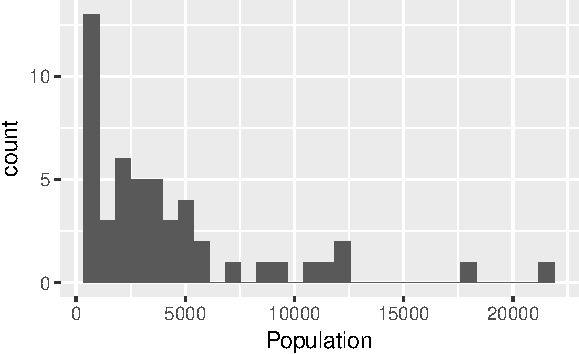
\includegraphics{pdaps_files/figure-latex/histogram-1}

Let's walk through the syntax there. In the first line, we call
\texttt{ggplot()}, specifying the data frame to draw from, then in the
\texttt{aes()} command (which stands for ``aesthetic'') we specify the
variable to plot. If this were a bivariate analysis, here we would have
also specified a \texttt{y} variable to put on the y-axis. If we had
just stopped there, we would have a sad, empty plot. The \texttt{+}
symbol indicates that we'll be adding something to the plot.
\texttt{geom\_histogram()} is the command to overlay a histogram.

We'll only be looking at a few of the ggplot commands today. I recommend
taking a look at the online package documentation at
\url{http://docs.ggplot2.org} to see all of the many features available.

When you're just making graphs for yourself to explore the data, you
don't need to worry about things like axis labels as long as you can
comprehend what's going on. But when you prepare graphs for others to
read (including those of us grading your problem sets!) you need to
include an informative title and axis labels. To that end, use the
\texttt{xlab()}, \texttt{ylab()}, and \texttt{ggtitle()} commands.

\begin{Shaded}
\begin{Highlighting}[]
\KeywordTok{ggplot}\NormalTok{(state_data, }\KeywordTok{aes}\NormalTok{(}\DataTypeTok{x =} \NormalTok{Population)) +}\StringTok{ }\KeywordTok{geom_histogram}\NormalTok{() +}\StringTok{ }
\StringTok{    }\KeywordTok{xlab}\NormalTok{(}\StringTok{"Population (thousands)"}\NormalTok{) +}\StringTok{ }\KeywordTok{ylab}\NormalTok{(}\StringTok{"Number of states"}\NormalTok{) +}\StringTok{ }
\StringTok{    }\KeywordTok{ggtitle}\NormalTok{(}\StringTok{"Some states are big, but most are small"}\NormalTok{)}
\end{Highlighting}
\end{Shaded}

\begin{verbatim}
## `stat_bin()` using `bins = 30`. Pick
## better value with `binwidth`.
\end{verbatim}

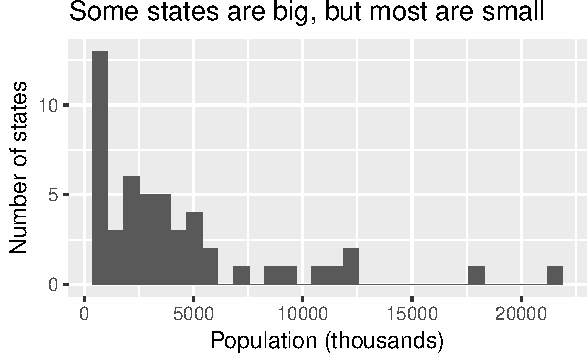
\includegraphics{pdaps_files/figure-latex/axis-labeling-1}

The density plot is a close relative of the histogram. It provides a
smooth estimate of the probability density function of the data.
Accordingly, the area under the density plot integrates to one.
Depending on your purposes, this can make the y-axis of a density plot
easier or (usually) harder to interpret than the count given by a
histogram.

\begin{Shaded}
\begin{Highlighting}[]
\KeywordTok{ggplot}\NormalTok{(state_data, }\KeywordTok{aes}\NormalTok{(}\DataTypeTok{x =} \NormalTok{Population)) +}\StringTok{ }\KeywordTok{geom_density}\NormalTok{()}
\end{Highlighting}
\end{Shaded}

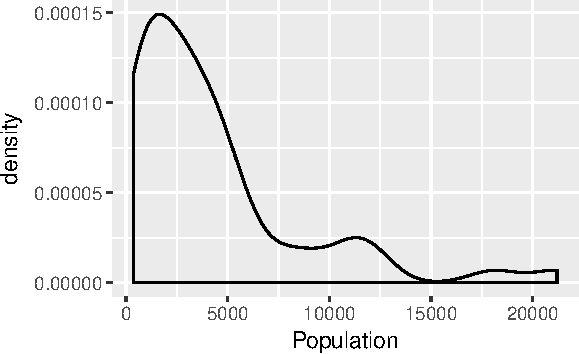
\includegraphics{pdaps_files/figure-latex/density-1}

The box plot is a common way to look at the distribution of a continuous
variable across different levels of a categorical variable.

\begin{Shaded}
\begin{Highlighting}[]
\KeywordTok{ggplot}\NormalTok{(state_data, }\KeywordTok{aes}\NormalTok{(}\DataTypeTok{x =} \NormalTok{Region, }\DataTypeTok{y =} \NormalTok{Population)) +}\StringTok{ }
\StringTok{    }\KeywordTok{geom_boxplot}\NormalTok{()}
\end{Highlighting}
\end{Shaded}

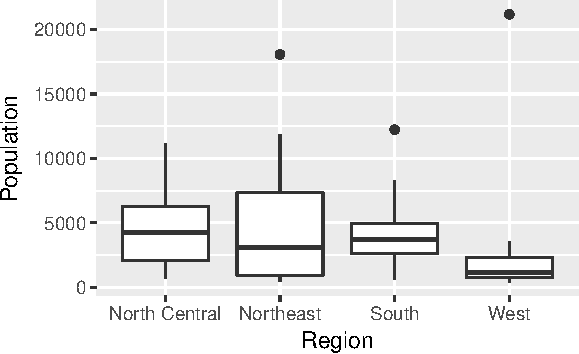
\includegraphics{pdaps_files/figure-latex/boxplot-1}

A box plot consists of the following components:

\begin{itemize}
\tightlist
\item
  Center line: median of the data
\item
  Bottom of box: 25th percentile
\item
  Top of box: 75th percentile
\item
  Lower ``whisker'': range of observations no more than 1.5 IQR (height
  of box) below the 25th percentile
\item
  Upper ``whisker'': range of observations no more than 1.5 IQR above
  the 75th percentile
\item
  Plotted points: any data lying outside the whiskers
\end{itemize}

If you want to skip the summary and plot the full distribution of a
variable across categories, you can use a violin plot.

\begin{Shaded}
\begin{Highlighting}[]
\KeywordTok{ggplot}\NormalTok{(state_data, }\KeywordTok{aes}\NormalTok{(}\DataTypeTok{x =} \NormalTok{Region, }\DataTypeTok{y =} \NormalTok{Population)) +}\StringTok{ }
\StringTok{    }\KeywordTok{geom_violin}\NormalTok{()}
\end{Highlighting}
\end{Shaded}

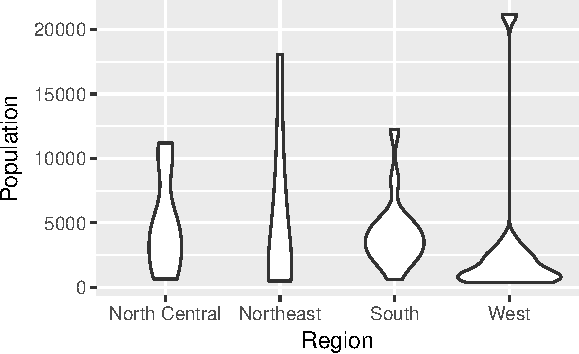
\includegraphics{pdaps_files/figure-latex/violin-1}

Technically, violin plots convey more information than box plots since
they show the full distribution. However, readers aren't as likely to be
familiar with a violin plot. It's harder to spot immediately where the
median is (though you could add that to the plot if you wanted). Plus,
violin plots look goofy with outliers---see the ``West'' column
above---whereas box plots handle them easily.

For visualizing relationships between continuous variables, nothing
beats the scatterplot.

\begin{Shaded}
\begin{Highlighting}[]
\KeywordTok{ggplot}\NormalTok{(state_data, }\KeywordTok{aes}\NormalTok{(}\DataTypeTok{x =} \NormalTok{Illiteracy, }\DataTypeTok{y =} \NormalTok{LifeExp)) +}\StringTok{ }
\StringTok{    }\KeywordTok{geom_point}\NormalTok{()}
\end{Highlighting}
\end{Shaded}

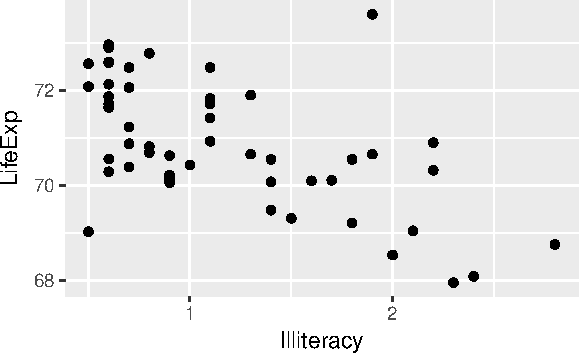
\includegraphics{pdaps_files/figure-latex/scatter-1}

When you're plotting states or countries, a hip thing to do is plot
abbreviated names instead of points. To do that, you can use
\texttt{geom\_text()} instead of \texttt{geom\_point()}, supplying an
additional aesthetic argument telling ggplot where to draw the labels
from.

\begin{Shaded}
\begin{Highlighting}[]
\KeywordTok{ggplot}\NormalTok{(state_data, }\KeywordTok{aes}\NormalTok{(}\DataTypeTok{x =} \NormalTok{Illiteracy, }\DataTypeTok{y =} \NormalTok{LifeExp)) +}\StringTok{ }
\StringTok{    }\KeywordTok{geom_text}\NormalTok{(}\KeywordTok{aes}\NormalTok{(}\DataTypeTok{label =} \NormalTok{Abbrev))}
\end{Highlighting}
\end{Shaded}

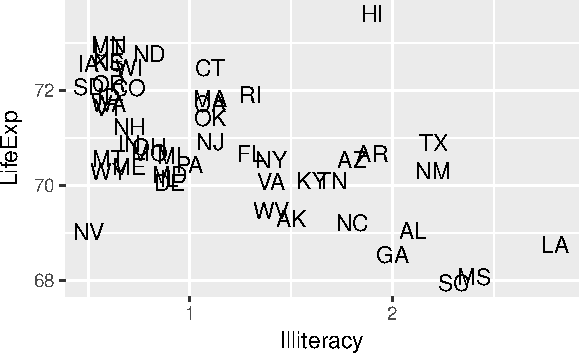
\includegraphics{pdaps_files/figure-latex/scatter-text-1}

Maybe it's overwhelming to look at all that raw data and you just want a
summary. For example, maybe you want an estimate of expected
\texttt{LifeExp} for each value of \texttt{Illiteracy}. This is called
the \emph{conditional expectation} and will be the subject of much of
the rest of the course. For now, just now that you can calculate a
smoothed conditional expectation via \texttt{geom\_smooth()}.

\begin{Shaded}
\begin{Highlighting}[]
\KeywordTok{ggplot}\NormalTok{(state_data, }\KeywordTok{aes}\NormalTok{(}\DataTypeTok{x =} \NormalTok{Illiteracy, }\DataTypeTok{y =} \NormalTok{LifeExp)) +}\StringTok{ }
\StringTok{    }\KeywordTok{geom_smooth}\NormalTok{()}
\end{Highlighting}
\end{Shaded}

\begin{verbatim}
## `geom_smooth()` using method = 'loess'
\end{verbatim}

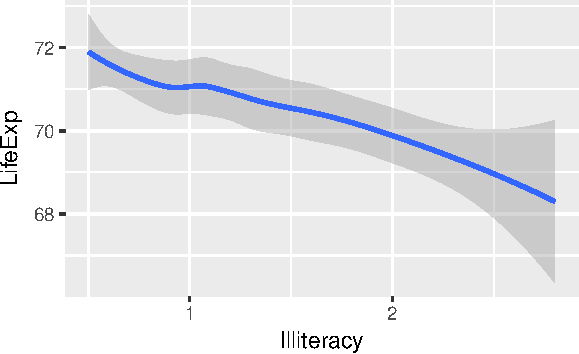
\includegraphics{pdaps_files/figure-latex/smooth-1}

And if you're the kind of overachiever who likes to have the raw data
\emph{and} the summary, you can do it. Just add them both to the
\texttt{ggplot()} call.

\begin{Shaded}
\begin{Highlighting}[]
\KeywordTok{ggplot}\NormalTok{(state_data, }\KeywordTok{aes}\NormalTok{(}\DataTypeTok{x =} \NormalTok{Illiteracy, }\DataTypeTok{y =} \NormalTok{LifeExp)) +}\StringTok{ }
\StringTok{    }\KeywordTok{geom_smooth}\NormalTok{() +}\StringTok{ }\KeywordTok{geom_point}\NormalTok{()}
\end{Highlighting}
\end{Shaded}

\begin{verbatim}
## `geom_smooth()` using method = 'loess'
\end{verbatim}

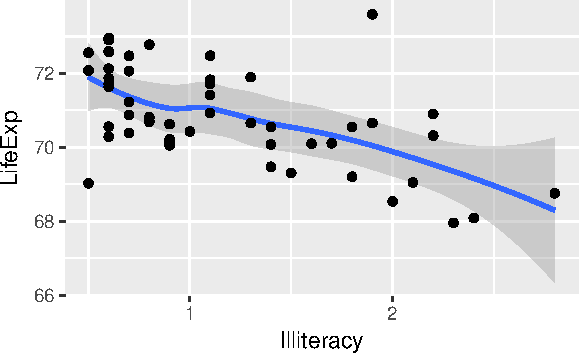
\includegraphics{pdaps_files/figure-latex/combine-1}

\section{Saving Plots}\label{saving-plots}

When you're writing in R Markdown, the plots go straight into your
document without much fuss. Odds are, your dissertation will contain
plots but won't be written in R Markdown, which means you'll need to
learn how to save them.

It's pretty simple:

\begin{enumerate}
\def\labelenumi{\arabic{enumi}.}
\tightlist
\item
  Assign your \texttt{ggplot()} call to a variable.
\item
  Pass that variable to the \texttt{ggsave()} function.
\end{enumerate}

\begin{Shaded}
\begin{Highlighting}[]
\NormalTok{pop_hist <-}\StringTok{ }\KeywordTok{ggplot}\NormalTok{(state_data, }\KeywordTok{aes}\NormalTok{(}\DataTypeTok{x =} \NormalTok{Population)) +}\StringTok{ }
\StringTok{    }\KeywordTok{geom_histogram}\NormalTok{()}

\KeywordTok{ggsave}\NormalTok{(}\DataTypeTok{filename =} \StringTok{"pop-hist.pdf"}\NormalTok{, }\DataTypeTok{plot =} \NormalTok{pop_hist, }
    \DataTypeTok{width =} \DecValTok{6}\NormalTok{, }\DataTypeTok{height =} \DecValTok{3}\NormalTok{)}
\end{Highlighting}
\end{Shaded}

If you want plot types other than PDF, just set a different extension.
See \texttt{?ggsave} for the possibilities.

\section{Faceting}\label{faceting}

Suppose you want to split the data into subgroups, as defined by some
variable in the data (e.g., the region states are in), and make the same
plot for each subgroup. ggplot's \emph{faceting} functions,
\texttt{facet\_wrap()} and \texttt{facet\_grid()}, make this easy.

To split up plots according to a single grouping variable, use
\texttt{facet\_wrap()}. This uses R's \emph{formula} syntax, defined by
the tilde \texttt{\textasciitilde{}}, which you'll become well
acquainted with once we start running regressions.

\begin{Shaded}
\begin{Highlighting}[]
\KeywordTok{ggplot}\NormalTok{(state_data, }\KeywordTok{aes}\NormalTok{(}\DataTypeTok{x =} \NormalTok{Population)) +}\StringTok{ }\KeywordTok{geom_histogram}\NormalTok{() +}\StringTok{ }
\StringTok{    }\KeywordTok{facet_wrap}\NormalTok{(~Region)}
\end{Highlighting}
\end{Shaded}

\begin{verbatim}
## `stat_bin()` using `bins = 30`. Pick
## better value with `binwidth`.
\end{verbatim}

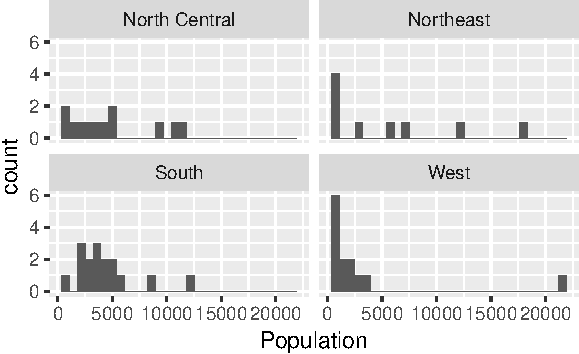
\includegraphics{pdaps_files/figure-latex/facet-wrap-1}

If you don't like the default arrangement, use the \texttt{ncol}
argument.

\begin{Shaded}
\begin{Highlighting}[]
\KeywordTok{ggplot}\NormalTok{(state_data, }\KeywordTok{aes}\NormalTok{(}\DataTypeTok{x =} \NormalTok{Population)) +}\StringTok{ }\KeywordTok{geom_histogram}\NormalTok{() +}\StringTok{ }
\StringTok{    }\KeywordTok{facet_wrap}\NormalTok{(~Region, }\DataTypeTok{ncol =} \DecValTok{1}\NormalTok{)}
\end{Highlighting}
\end{Shaded}

\begin{verbatim}
## `stat_bin()` using `bins = 30`. Pick
## better value with `binwidth`.
\end{verbatim}

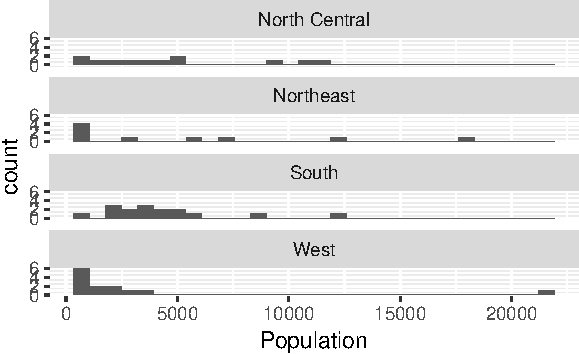
\includegraphics{pdaps_files/figure-latex/facet-wrap-ncol-1}

For two grouping variables, use \texttt{facet\_grid()}, putting
variables on both sides of the formula.

\begin{Shaded}
\begin{Highlighting}[]
\KeywordTok{ggplot}\NormalTok{(state_data, }\KeywordTok{aes}\NormalTok{(}\DataTypeTok{x =} \NormalTok{Population)) +}\StringTok{ }\KeywordTok{geom_histogram}\NormalTok{() +}\StringTok{ }
\StringTok{    }\KeywordTok{facet_grid}\NormalTok{(Region ~}\StringTok{ }\NormalTok{IncomeGroup)}
\end{Highlighting}
\end{Shaded}

\begin{verbatim}
## `stat_bin()` using `bins = 30`. Pick
## better value with `binwidth`.
\end{verbatim}

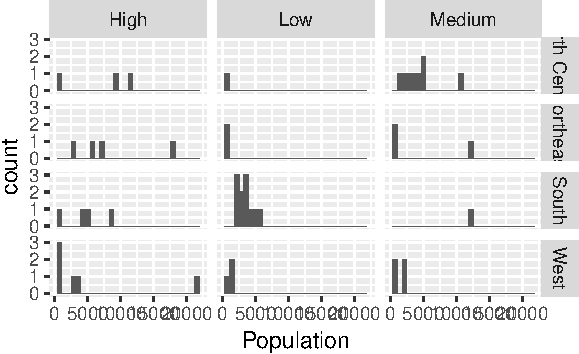
\includegraphics{pdaps_files/figure-latex/facet-grid-1}

\section{Aesthetics}\label{aesthetics}

Faceting is one way to incorporate information about additional
variables into what would otherwise be a plot of just one or two
variables. Aesthetics---which alter the appearance of particular plot
features depending on the value of a variable---provide another way to
do that.

For example, when visualizing the relationship between statewide
illiteracy and life expectancy, you might want larger states to get more
visual weight. You can set the \texttt{size} aesthetic of the
\texttt{point} geometry to vary according to the state's population.

\begin{Shaded}
\begin{Highlighting}[]
\KeywordTok{ggplot}\NormalTok{(state_data, }\KeywordTok{aes}\NormalTok{(}\DataTypeTok{x =} \NormalTok{Illiteracy, }\DataTypeTok{y =} \NormalTok{LifeExp)) +}\StringTok{ }
\StringTok{    }\KeywordTok{geom_point}\NormalTok{(}\KeywordTok{aes}\NormalTok{(}\DataTypeTok{size =} \NormalTok{Population))}
\end{Highlighting}
\end{Shaded}

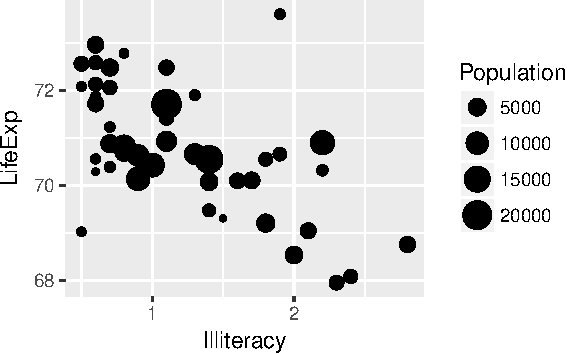
\includegraphics{pdaps_files/figure-latex/aes-size-1}

The \textbf{ggplot2} documentation lists the available aesthetics for
each function. Another popular one is \texttt{colour}, which is great
for on-screen display but not so much for the printed page. (And
terrible for the colorblind!)

\begin{Shaded}
\begin{Highlighting}[]
\KeywordTok{ggplot}\NormalTok{(state_data, }\KeywordTok{aes}\NormalTok{(}\DataTypeTok{x =} \NormalTok{Illiteracy, }\DataTypeTok{y =} \NormalTok{LifeExp)) +}\StringTok{ }
\StringTok{    }\KeywordTok{geom_point}\NormalTok{(}\KeywordTok{aes}\NormalTok{(}\DataTypeTok{colour =} \NormalTok{Region))}
\end{Highlighting}
\end{Shaded}

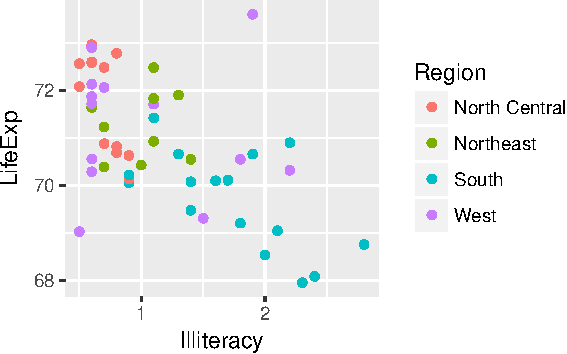
\includegraphics{pdaps_files/figure-latex/aes-colour-1}

For line graphs or density plots, you can set the \texttt{linetype} to
vary by category.

\begin{Shaded}
\begin{Highlighting}[]
\KeywordTok{ggplot}\NormalTok{(state_data, }\KeywordTok{aes}\NormalTok{(}\DataTypeTok{x =} \NormalTok{Population)) +}\StringTok{ }\KeywordTok{geom_density}\NormalTok{(}\KeywordTok{aes}\NormalTok{(}\DataTypeTok{linetype =} \NormalTok{IncomeGroup))}
\end{Highlighting}
\end{Shaded}

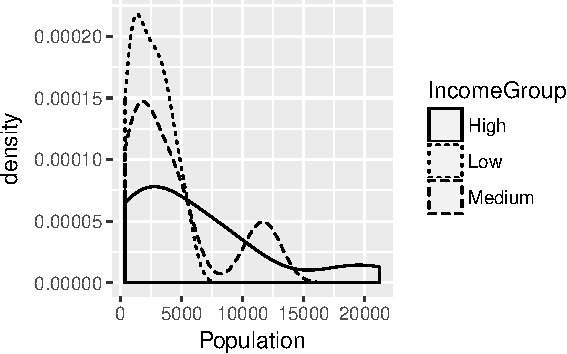
\includegraphics{pdaps_files/figure-latex/aes-linetype-1}

(I always find these incomprehensible with more than two lines, but
maybe that's just me.) You can use multiple aesthetics together, and you
can even combine aesthetics with faceting, as in the following example.

\begin{Shaded}
\begin{Highlighting}[]
\KeywordTok{ggplot}\NormalTok{(state_data, }\KeywordTok{aes}\NormalTok{(}\DataTypeTok{x =} \NormalTok{Illiteracy, }\DataTypeTok{y =} \NormalTok{LifeExp)) +}\StringTok{ }
\StringTok{    }\KeywordTok{geom_smooth}\NormalTok{() +}\StringTok{ }\KeywordTok{geom_text}\NormalTok{(}\KeywordTok{aes}\NormalTok{(}\DataTypeTok{label =} \NormalTok{Abbrev, }
    \DataTypeTok{colour =} \NormalTok{Region, }\DataTypeTok{size =} \NormalTok{Population)) +}\StringTok{ }\KeywordTok{facet_wrap}\NormalTok{(~IncomeGroup)}
\end{Highlighting}
\end{Shaded}

\begin{verbatim}
## `geom_smooth()` using method = 'loess'
\end{verbatim}

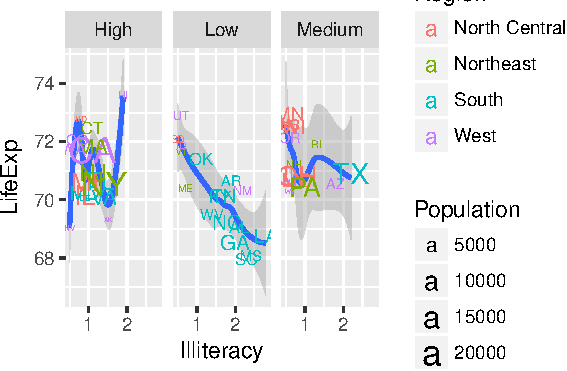
\includegraphics{pdaps_files/figure-latex/too-many-things-1}

But the fact that you \emph{can} do something doesn't mean you
\emph{should}. That plot is so cluttered that it's hard to extract the
relevant information from it. Data visualizations should communicate a
clear message to viewers without overwhelming them. To do this well
takes practice, patience, and maybe even a bit of taste.

\section{Appendix: Creating the Example
Data}\label{appendix-creating-the-example-data-1}

The example data comes from data on U.S. states in 1977 that are
included with base R. See \texttt{?state}.

\begin{Shaded}
\begin{Highlighting}[]
\KeywordTok{library}\NormalTok{(}\StringTok{"tidyverse"}\NormalTok{)}

\NormalTok{state_data <-}\StringTok{ }\NormalTok{state.x77 %>%}\StringTok{ }\KeywordTok{as_tibble}\NormalTok{() %>%}\StringTok{ }\KeywordTok{add_column}\NormalTok{(}\DataTypeTok{State =} \KeywordTok{rownames}\NormalTok{(state.x77), }
    \DataTypeTok{Abbrev =} \NormalTok{state.abb, }\DataTypeTok{Region =} \NormalTok{state.region, }
    \DataTypeTok{.before =} \DecValTok{1}\NormalTok{) %>%}\StringTok{ }\KeywordTok{rename}\NormalTok{(}\DataTypeTok{LifeExp =} \StringTok{`}\DataTypeTok{Life Exp}\StringTok{`}\NormalTok{, }
    \DataTypeTok{HSGrad =} \StringTok{`}\DataTypeTok{HS Grad}\StringTok{`}\NormalTok{) %>%}\StringTok{ }\KeywordTok{mutate}\NormalTok{(}\DataTypeTok{IncomeGroup =} \KeywordTok{cut}\NormalTok{(Income, }
    \DataTypeTok{breaks =} \KeywordTok{quantile}\NormalTok{(Income, }\DataTypeTok{probs =} \KeywordTok{seq}\NormalTok{(}\DecValTok{0}\NormalTok{, }\DecValTok{1}\NormalTok{, }
        \DataTypeTok{by =} \DecValTok{1}\NormalTok{/}\DecValTok{3}\NormalTok{)), }\DataTypeTok{labels =} \KeywordTok{c}\NormalTok{(}\StringTok{"Low"}\NormalTok{, }\StringTok{"Medium"}\NormalTok{, }
        \StringTok{"High"}\NormalTok{), }\DataTypeTok{include.lowest =} \OtherTok{TRUE}\NormalTok{))}

\KeywordTok{write_csv}\NormalTok{(state_data, }\DataTypeTok{path =} \StringTok{"state-data.csv"}\NormalTok{)}
\end{Highlighting}
\end{Shaded}

\bibliography{packages.bib,book.bib,psci-8357.bib}



\end{document}
